% (c) 2012 -2014 Dimitrios Vrettos - d.vrettos@gmail.com
% (c) 2014 Claudio Carboncini - claudio.carboncini@gmail.com
% (c) 2014 Daniele Zambelli - daniele.zambelli@gmail.com

\chapter{Numeri naturali}

\section{L'origine dei numeri}
\label{sec:01_origine}

L'origine del sistema dei numeri naturali si perde nella notte dei tempi. 
Non abbiamo documenti sufficienti per capire come l'uomo li abbia costruiti o 
scoperti; è possibile che il nostro sistema di numerazione sia nato 
contemporaneamente al linguaggio stesso della specie umana. 
Sono stati ritrovati reperti fossili risalenti a più di trentamila
anni fa, recanti delle incisioni a distanza regolare. 
In particolare, è stato ritrovato un osso di babbuino, detto “Osso di Ishango” 
(figura \ref{fig:ishango}) 
\footnote{\url{http://it.wikipedia.org/wiki/Osso_d'Ishango}} 
in quanto è stato rinvenuto presso la città di Ishango nel Congo tra il Nilo 
e il lago Edoardo, che riporta delle tacche disposte in modo tale da farci 
pensare che rappresentino dei numeri o dei calcoli. L'osso risale a
un periodo tra il~20\,000\,~\aC~e il~18\,000\,~\aC

\begin{wrapfloat}{figure}{r}{0pt}
\begin{inaccessibleblock}[Descrizione immagine: Osso con incise alcune tacche regolari]
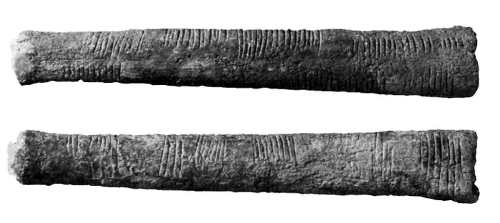
\includegraphics[scale=0.35]{img/fig001.png}
\end{inaccessibleblock}
\caption{Osso di Ishango}
\label{fig:ishango}
\end{wrapfloat}

Possiamo immaginare che i pastori per contare i capi del proprio gregge, 
facessero delle tacche su dei bastoni mano a mano che le pecore entravano nel 
recinto una alla volta: una tacca per ogni pecora. 
Tuttavia, questo metodo di associazione uno ad uno (una tacca per una pecora) 
non è efficace per greggi, o oggetti da contare, di grandi dimensioni. 
Si immagini, per esempio, la difficoltà di tracciare cinquecento tacche su un 
bastone. 
È possibile allora che per rappresentare numeri grandi si siano cominciati a 
usare simboli specifici che richiamassero alla mente i numeri grandi e che 
contemporaneamente siano state fissate alcune regole per associare questi 
simboli.

Sappiamo per certo che circa~6\,000 anni fa gli antichi Egizi scrivevano, 
incidendo sulla pietra, i numeri utilizzando geroglifici per le potenze di~10:

% % (c) 2012 Dimitrios Vrettos - d.vrettos@gmail.com
% Numeri egiziani
\begin{table}[!h]
  \begin{center}
    \begin{tabular}{ccccccc}
      \toprule
	\begin{hieroglyph}{\leavevmode \loneSign{\Aca GC/42/}}\end{hieroglyph} &  %
	\begin{hieroglyph}{\leavevmode \loneSign{\Aca GI/40/}}\end{hieroglyph} &%
	\begin{hieroglyph}{\leavevmode \loneSign{\Aca GD/84/}}\end{hieroglyph} &%
	\begin{hieroglyph}{\leavevmode \loneSign{\Aca GM/43/}}\end{hieroglyph} &%
	\begin{hieroglyph}{\leavevmode \loneSign{\Aca GV/32/}}\end{hieroglyph} &%
	\begin{hieroglyph}{\leavevmode \loneSign{\Aca GV/51/}}\end{hieroglyph}&%
	\begin{hieroglyph}{\leavevmode \loneSign{\Aca GZ/32/}}\end{hieroglyph}\\
      \midrule
	1\,000\,000   & 100\,000 & 10\,000 & 1\,000 & 100 & 10 & 1\\
      \bottomrule
    \end{tabular}
  \end{center}
\end{table}
\begin{inaccessibleblock}[Descrizione immagine: Geroglifici che rappresentano le potenze di 10 da uno a un milione]
\vspace{-2ex}
\begin{center} 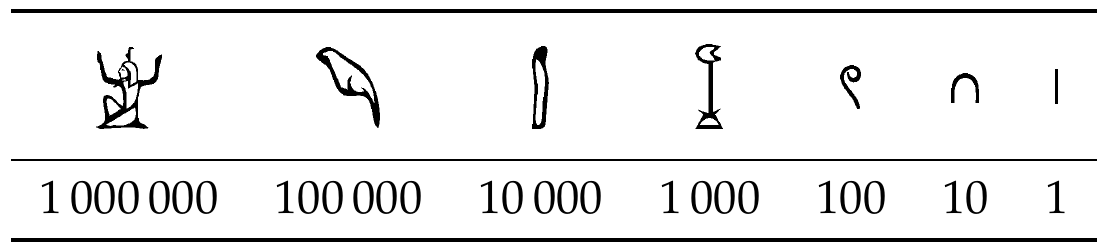
\includegraphics[scale=0.28]{img/hieropotdieci.png} \end{center}
\vspace{-2ex}
\end{inaccessibleblock}
                                                                  
Ripetendo questi simboli è possibile scrivere, per esempio, il numero~3673 
così:

% \vspace{-2ex}% (c) 2012 Dimitrios Vrettos - d.vrettos@gmail.com
  \begin{center}
    \begin{hieroglyph}{\leavevmode \loneSign{\Aca GM/43/}\HinterSignsSpace
\loneSign{\Aca GM/43/}\HinterSignsSpace
\loneSign{\Aca GM/43/}\HinterSignsSpace
\Cadrat{\CadratLineI{\Aca GV/32/\hfill\Aca GV/32/\hfill\Aca GV/32/}\CadratLine{\Aca GV/32/\hfill\Aca GV/32/\hfill\Aca GV/32/}}\HinterSignsSpace
\Cadrat{\CadratLineI{{\Hsmaller\Hsmaller\Aca GV/51/}\hfill{\Hsmaller\Hsmaller\Aca GV/51/}\hfill{\Hsmaller\Hsmaller\Aca GV/51/}}\CadratLine{\Aca GV/51/\hfill\Aca GV/51/\hfill\Aca GV/51/\hfill\Aca GV/51/}}\HinterSignsSpace
\loneSign{\Aca GZ/32/}\HinterSignsSpace
\loneSign{\Aca GZ/32/}\HinterSignsSpace
\loneSign{\Aca GZ/32/}}\end{hieroglyph}
  \end{center}\vspace{-2ex}
\begin{inaccessibleblock}[Descrizione immagine: Numero 3673 scritto con i geroglifici]
\vspace{-2ex}
\begin{center} 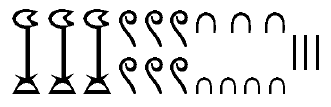
\includegraphics[scale=0.25]{img/hiero3673.png} \end{center}
\vspace{-2ex}
\end{inaccessibleblock}

I Romani usavano invece sette simboli con i quali, seguendo determinate 
regole, rappresentavano qualunque numero. 
I simboli sono~$I=1$, $V=5$, $X=10$, $L=50$, $C=100$, $D=500$, $M=1000$.
Il numero~$MM$ rappresenta~$~1000+1000 =~2000$; il numero~$ VI$ 
rappresenta~$~5+1=6~$, mentre il numero~$ IV~$ rappresenta~$~5-1=4~$.

\section{I numeri naturali}
\label{sec:01_naturali}

I primi numeri che abbiamo usato sin da bambini per contare gli oggetti o le 
persone si chiamano \emph{numeri naturali}
\[ 0, 1, 2, 3, 4, 5, 6, 7, 8, 9, 10, 11, 12, 13\dots \]
L'insieme di tutti questi numeri si indica con la lettera~$\insN$.

Cosa hanno in comune le dita di una mano, con~5 mele,~5~penne,~5~sedie? 
Evidentemente il numero~5. Una caratteristica cioè che è comune a tutti gli 
insiemi formati da~5 oggetti. 
Questa caratteristica può essere vista come un oggetto a sé stante, 
un oggetto astratto di tipo matematico.

Ma i numeri naturali non servono solo per indicare quanti oggetti ci sono 
(aspetto \emph{cardinale} del numero), vengono usati anche per rappresentare 
l'ordine con cui si presentano gli oggetti, (aspetto \emph{ordinale}), 
l'ordine per esempio con cui i corridori arrivano al traguardo: primo, 
secondo, terzo, \ldots

Nonostante i numeri naturali e le operazioni su di essi ci vengano insegnati 
fin da piccoli, e nonostante l'umanità li usi da tempi antichissimi una loro 
piena comprensione non è semplice, come dimostra il fatto che ancora oggi i 
matematici ne discutono. 
Il dibattito su cosa sono i numeri e su cosa si fondano è stato 
particolarmente animato nei primi decenni del $XX$~secolo, quando ne hanno 
discusso matematici e filosofi come Frege, Peano, Russell, Hilbert e tanti 
altri. Oggi ci sono diversi punti di vista.

\section{Cosa sono}
\label{sec:01_definizione}

I numeri naturali sono alla base dell'aritmetica, 
tutti gli altri numeri si possono costruire a partire da questi. 
Chiederci cosa sono i numeri naturali non è una domanda da poco, 
è domandarsi che cosa sono quegli oggetti su cui poggia una gran parte della
matematica.

Per definire i numeri naturali dobbiamo partire da alcuni 
\emph{concetti primitivi}. 
I concetti primitivi sono dei concetti che decidiamo di non definire e che 
siamo tutti d'accordo di ritenere conosciuti.

I concetti primitivi per definire i numeri naturali sono:

\begin{itemize*}
 \item lo zero;
 \item il successore di un numero.
\end{itemize*}

Lo \emph{zero} è il numero che serve per contare gli elementi di un insieme 
con il minore numero di elementi possibile: l'insieme vuoto.

Il \emph{successore} di un numero naturale~$n$ è quel numero che viene subito 
dopo~$n$.

Quindi se siamo d'accordo su questi due concetti di base, possiamo definire i 
numeri naturali come un insieme nel quale valgono le seguenti proprietà:

\begin{enumerate*}
 \item Zero è un numero naturale.
 \item Per ogni numero naturale, anche il suo successore è un numero naturale.
 \item Numeri diversi hanno successori diversi.
 \item Lo zero non è successore di nessun numero naturale.
 \item Se una proprietà vale per lo zero e, 
   valendo per un numero naturale qualsiasi, 
   vale anche per il suo successore 
   allora vale per ogni numero naturale.
\end{enumerate*}

In pratica i numeri naturali sono la sequenza:

 zero, uno, due, tre, ... centoventitre, centoventiquattro, ...

Un modo comodo per esprimere qualunque numero naturale è usare dei segni 
appositi, le cifre, e un sistema per rappresentarli:

 0, 1, 2, 3, ... 123, 124, ...

\section{Il sistema di numerazione decimale posizionale}
\label{sec:01_sist10}

Il modo di scrivere i numeri dei romani risultava piuttosto complicato sia 
nella scrittura dei numeri sia nell'esecuzione dei calcoli. 
Il sistema moderno di scrittura dei numeri fa uso dei soli dieci 
simboli~0, 1, 2, 3, 4, 5, 6, 7, 8, 9, che vengono detti \emph{cifre}.
Un numero non è altro che una sequenza ordinata di cifre, eventualmente 
ripetute.

Per rappresentare il numero dieci che segue il~9 non si fa uso di un simbolo 
diverso ma si scrivono due cifre: il simbolo~1 a sinistra e il simbolo~0 a 
destra. 
Per chiarire questo metodo utilizziamo un pallottoliere 
(figura \ref{fig:pallottoliere}) con aste verticali capaci di contenere 
fino a~9 dischetti: per rappresentare il numero~10 dispongo un dischetto 
nell'asta a sinistra e vuoto la prima asta: 
il numero dieci viene rappresentato dalla scrittura~10.

\begin{inaccessibleblock}[Pallottoliere]
\begin{figure}[h]
\begin{center}
% (c) 2012 Dimitrios Vrettos - d.vrettos@gmail.com
% pallottoliere

\newcommand{\base}{%
  \filldraw[fill=black!90, draw=gray!80,rounded corners,shading=radial, inner color=white, outer color=gray!90]%
    (-2.4cm, -0.2cm) rectangle (2.4cm,0.4cm);
}

\newcommand{\aste}{%
  \fill[fill=black!90,rounded corners,shading=radial, inner color=white, outer color=gray!90]%
    (-1.25mm,3mm) rectangle (1.25mm,4.3cm);
}

\newcommand{\disco}{%
    \filldraw[fill=gray!20,draw=gray, rounded corners, shade,shading=radial, inner color=white, outer color=blue!50]%
      (-.6cm, .4cm) rectangle (.6cm,0.8cm);
}
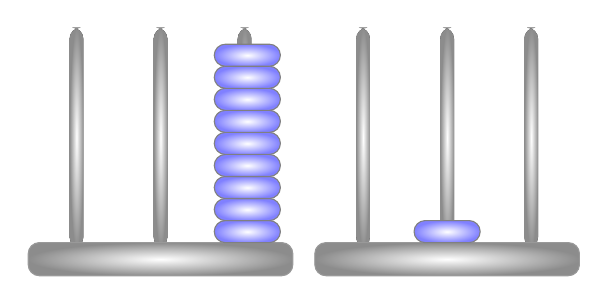
\begin{tikzpicture}[scale=.7]
  \foreach \n/\a in {-15.25mm,0,15.25mm,36.75mm,52mm,67.25mm}{
    \begin{scope}[xshift=\a]
      \aste
    \end{scope}
  }

  \foreach \n/\x in {1/0cm,2/5.2cm}{%
    \begin{scope}[xshift=\x]
	\base
    \end{scope}
  }
  
  \foreach \n/\y in {0,.4cm,...,3.2cm}{%
    \begin{scope}[xshift=15.75mm,yshift=\y]
	\disco
    \end{scope}
  }   	
	
  \foreach \n/\z in {0}{%
    \begin{scope}[xshift=52mm,yshift=\z]
      \disco
    \end{scope}
  }

\end{tikzpicture}

\caption{Il pallottoliere}
\label{fig:pallottoliere}
\end{center}
\end{figure}
\end{inaccessibleblock}

 
I dischetti sull'ultima asta rappresentano il numero~9; un dischetto sulla 
penultima rappresenta il numero~10. 
Per rappresentare il numero cento si fa uso della scrittura~100.
Ovvero si sposta il numero~1 ancora a sinistra ponendo uno zero nel posto 
lasciato vuoto.
Questo metodo può essere ripetuto per rappresentare tutti i numeri che 
risultino potenza di dieci, ovvero dieci, cento, mille\ldots

Le potenze di~10 sono importanti nel sistema decimale poiché rappresentano 
il peso di ciascuna cifra di cui è composto il numero. 
Nel pallottoliere ciascuna asta indica una potenza di dieci. 
Il valore di un numero si ottiene moltiplicando ciascuna cifra per il
suo peso e sommando i valori ottenuti.

Per esempio, tre dischetti nella terza asta rappresentano il 
numero~$~3\cdot 10^2=300$.
Il numero~$219$ si rappresenta tenendo conto di questa 
scrittura~$~2\cdot 10^2+1\cdot 10+9$.

Per quanto detto, il sistema di numerazione che usiamo è:

\begin{itemize*}
 \item \emph{decimale} o a base dieci, 
  perché usiamo dieci segni (cifre) per scrivere i numeri;
 \item \emph{posizionale} 
  perché una stessa cifra assume un peso (valore) diverso a seconda della 
  posizione che occupa.
\end{itemize*}

\subsection{Rappresentazione geometrica}
I numeri naturali possono essere rappresentati su una semiretta: 
si identifica il numero~0 con l'origine della semiretta, come verso di 
percorrenza si prende quello da sinistra verso destra e come unità di misura 
un segmento~$AB$. 
Si riporta questa unità di misura più volte partendo dall'origine e a ogni 
passo si va al numero successivo.

\begin{inaccessibleblock}[Semiretta orientata con origine 0]
\begin{center}
 % (c) 2012 Dimitrios Vrettos - d.vrettos@gmail.com

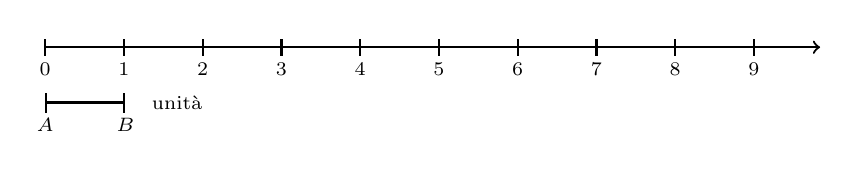
\begin{tikzpicture}
\begin{scope}[thick,font=\scriptsize]
	\draw[->] (0,0)  - -  (280pt,0) node[above]{$\insN$};
% 	\draw(1,-3pt) -- (1,3pt) node[below]{$1$};	
		\foreach \n in {0,1,2,...,9}{%
        	\draw (\n,-3pt) -- (\n,3pt)   node [below=5pt] {$\n$};}

		\draw[|-|]node [below=22pt]{$A$}(0,-20pt)--(29pt,-20pt) node[below=2pt]{$B$};

\end{scope}
\node [right,font=\scriptsize] at (+35pt,-20pt) {unit\`a};
\end{tikzpicture}

\end{center}
\end{inaccessibleblock}

Ogni numero naturale si costruisce a partire dal numero~0 e passando di volta 
in volta al numero successivo:~1 è il successore di~0,~2~è il successore 
di~1,~3~è il successore di~2, etc. 
Ogni numero naturale ha il successore e ogni numero, a eccezione di~0, ha il
precedente. 
L'insieme~$\insN$ ha~0 come elemento minimo e non ha un elemento massimo.

I numeri rappresentati sulla retta sono sempre più grandi man mano che si 
procede da sinistra verso destra. 
Ogni numero è maggiore di tutti i suoi precedenti, quelli che stanno alla sua 
sinistra, e minore di tutti i suoi successivi, quelli che stanno alla sua 
destra. 
Tra i numeri naturali esiste quindi una relazione d'ordine, che si rappresenta 
con il simbolo di 
\emph{disuguaglianza}~($\le$ si legge ``minore o uguale di'') o 
\emph{disuguaglianza stretta}~($<$ si legge ``minore di'').
Grazie a questo ordinamento, è sempre possibile confrontare due numeri 
naturali qualsiasi.

\begin{legge}[di tricotomia]
Dati due numeri naturali n, m vale sempre una delle seguenti tre relazioni: 
\quad n > m,\quad n < m,\quad n = m.
\end{legge}

\section{Operazioni con i numeri naturali}
\label{sec:01_operazioni}

Le operazioni matematiche sono delle regole che associano ad
alcuni oggetti matematici, gli \emph{operandi}, un altro oggetto matematico, 
il \emph{risultato}.

Di seguito riprendiamo rapidamente le prime cinque operazioni aritmetiche 
nei numeri naturali. 

\subsection{Proprietà delle operazioni}

Prima ancora di affrontare le operazioni aritmetiche con i numeri naturali, 
vediamo le proprietà delle operazioni in generale. \emph{In generale} vuol 
dire che ora non stiamo a precisare né di quale insieme numerico parliamo, 
né di quale operazione. Quindi useremo delle lettere per indicare  
operandi e  risultato mentre, per l'operazione, useremo un simbolo diverso 
da quelli delle quattro operazioni. Diremo che:

\begin{itemize*}
 \item Un'operazione si dice \emph{legge di composizione interna} se
  il risultato appartiene allo stesso insieme degli operandi.
 \item Un'operazione gode della proprietà \emph{commutativa} se 
  $a \star b = b \star a$
 \item Un'operazione gode della proprietà \emph{associativa} se 
  $(a \star b) \star c = a \star (b \star c)$
 \item Un'operazione possiede un \emph{elemento neutro} se 
  $a \star u = u \star a = a$
 \item Un'operazione possiede elemento \emph{inverso} se per ogni
  elemento $a$ dell'insieme, esiste un elemento $a'$ 
  dell'insieme per cui $a \star a' = a' \star a = u$ dove $u$ è l'elemento
  neutro.
\end{itemize*}

Vediamo ora alcune operazioni con i numeri naturali e le loro proprietà.

\subsection{Addizione in $\insN$}

Tra i numeri naturali è definita l'operazione di addizione come segue:

\begin{definizione}
  Dati due numeri naturali~$n$ e~$m$, l'\emph{addizione} associa un terzo 
  numero~$s$, che si ottiene partendo da~$n$ e procedendo verso i successivi 
  $m$~volte. Si scrive~$n+m=s$.
\end{definizione}

Ad esempio: sommare~5 a~3 significa partire da~3 e spostarsi verso il 
successivo per~5 volte.

\begin{minipage}{0.80\textwidth}
 \centering
 $3+5=8$

 % (c) 2012 Dimitrios Vrettos - d.vrettos@gmail.com

\begin{center}
 \begin{tikzpicture}[decoration={markings,mark=between positions 0.7 and .9 step 30pt with {\arrow{stealth}}}]
  \begin{scope}[thick,font=\scriptsize]
   \draw[->] (0,0)  - -  (280pt,0) node[above]{$\insN$};
    \foreach \c in {3,4,...,7}{%
     \draw[dotted, color=RedOrange,postaction={decorate}](\c,5pt)--(\c,5pt) arc (180:0:0.5 and 0.5);}
    \foreach \n in {0,1,2,...,9}{%	
     \draw (\n,-3pt) -- (\n,3pt)   node [below=5pt] {$\n$};}
  \end{scope}
 \end{tikzpicture}
\end{center}

\end{minipage}%
\begin{minipage}{0.15\textwidth}
 \centering
\begin{inaccessibleblock}[Descrizione immagine: semiretta dei numeri naturali sulla quale sono segnati spostamenti a destra di tre unit��]
 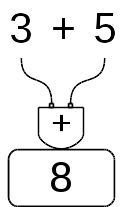
\includegraphics[scale=0.35]{img/op_add.png}
\end{inaccessibleblock}
\end{minipage}%

Gli operandi dell'addizione si chiamano \emph{addendi} e il risultato si 
chiama \emph{somma}.

\osservazione Per definire l'addizione abbiamo utilizzato il concetto di 
successore.

\subsubsection{Proprietà}

Per come è definita, e dato che i numeri naturali non hanno un limite 
superiore, l'addizione tra due numeri  naturali qualsiasi è sempre un numero
naturale. Si dice che è una \emph{legge di composizione interna}. 

Nei numeri naturali l'addizione presenta le seguenti proprietà:

\begin{itemize*}
 \item \emph{Commutativa}: $a + b = b + a$
 \item \emph{Associativa}: $(a + b) + c = a + (b + c)$
 \item \emph{Elemento neutro} $a + 0 = 0 + a = a$
\end{itemize*}

\subsection{Sottrazione in $\insN$}

Tra i numeri naturali è definita l'operazione di sottrazione come segue:

\begin{definizione}
Dati due numeri naturali~$m$ e~$n$, la sottrazione associa un terzo numero 
naturale~$d$, se esiste, che aggiunto ad~$n$ dà come somma~$m$.
Si scrive~$m - n = d$.
\end{definizione}

Ad esempio: togliere~5 da~7 significa partire da~7 e spostarsi verso il 
precedente per~5 volte.

\begin{minipage}{0.80\textwidth}
 \centering
 $7-5=2$ perché~$2+5=7$

 % (c) 2012 Dimitrios Vrettos - d.vrettos@gmail.com

\begin{center}
 \begin{tikzpicture}[decoration={markings,mark=between positions .3 and .5 step 30pt with {\arrowreversed{stealth}}}]
  \begin{scope}[thick,font=\scriptsize]
   \draw[->] (0,0)  - -  (280pt,0) node[above]{$\insN$};
    \foreach \c in {2,3,...,6}{%
     \draw[dotted, color=CornflowerBlue,postaction={decorate}](\c,5pt)--(\c,5pt) arc (180:0:0.5 and 0.5);}
    \foreach \n in {0,1,2,...,9}{%	
     \draw (\n,-3pt) -- (\n,3pt)   node [below=5pt] {$\n$};}
  \end{scope}
 \end{tikzpicture}
\end{center}

\end{minipage}%
\begin{minipage}{0.15\textwidth}
 \centering
\begin{inaccessibleblock}[Descrizione immagine: semiretta dei naturali con spostamenti a sinistra di 5 unit��]
 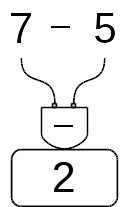
\includegraphics[scale=0.35]{img/op_sot.png}
\end{inaccessibleblock}
\end{minipage}%

Il primo operando si chiama \emph{minuendo}, il secondo \emph{sottraendo} e 
il risultato \emph{differenza}.

La sottrazione è l'operazione inversa dell'addizione.

Se al concetto di successivo aggiungiamo anche quello di precedente, possiamo 
definire la sottrazione anche in un altro modo.
Ritornando alla rappresentazione dei numeri naturali sulla semiretta 
orientata, la differenza tra i numeri~7 e~5 si può trovare partendo da~7 e 
procedendo a ritroso di~5 posizioni.

Diventa allora evidente perché non è possibile trovare la differenza 
tra~5 e~7, infatti se partendo dal~5 andiamo indietro di~7 posizioni 
usciamo dalla semiretta dei numeri naturali.

\begin{inaccessibleblock}[Descrizione immagine: semiretta dei numeri reali con spostamenti a sinistra oltre lo 0]
% (c) 2012 Dimitrios Vrettos - d.vrettos@gmail.com

\begin{center}
 \begin{tikzpicture}[decoration={markings,mark=between positions .3 and .5 step 30pt with {\arrowreversed{stealth}}}]
  \begin{scope}[thick,font=\scriptsize]
   \draw[->] (0,0)  - -  (280pt,0) node[above]{$\insN$};
    \foreach \c in {-2,-1,...,4}{%
     \draw[dotted, color=CornflowerBlue,postaction={decorate}](\c,5pt)--(\c,5pt) arc (180:0:0.5 and 0.5);}
    \foreach \n in {0,1,2,...,9}{%	
     \draw (\n,-3pt) -- (\n,3pt)   node [below=5pt] {$\n$};}
  \end{scope}
 \end{tikzpicture}
\end{center}

\end{inaccessibleblock}

Si può osservare allora che in~$\insN$ la sottrazione~$a - b$ è possibile solo 
se~$b\leq a$.

\osservazione Nella definizione di sottrazione abbiamo usato l'operazione di 
addizione.

\subsubsection{Proprietà}

Dato che non dà sempre un risultato, la sottrazione non è una 
\emph{legge di composizione interna} ai numeri naturali. 

Non è commutativa né associativa e non ha neppure un elemento neutro.
Possiamo dire che ha solo l'elemento neutro a destra infatti $a - 0 = a$, 
ma in generale non si può fare $0 - a$.

L'unica proprietà interessante della sottrazione è la proprietà 
\begin{itemize*}
 \item \emph{Invariantiva}: $a - b = (a \mp c) - (b \mp c)$
\end{itemize*}

Cioè: 
\begin{definizione}
aggiungendo o togliendo ad entrambi i termini di una sottrazione 
la stessa quantità la differenza non  cambia.
\end{definizione}

\subsection{Moltiplicazione in $\insN$}

Tra i numeri naturali è definita l'operazione di moltiplicazione come segue:

\begin{definizione}
Dati due numeri naturali~$m$,~$n$, l'operazione di \emph{moltiplicazione} 
associa un terzo numero~$p$ che si ottiene sommando~$n$ addendi tutti uguali 
a~$m$:

\begin{inaccessibleblock}[
$$m \times n = \mbox{n volte}{(m + m + \dots + m)} = p$$
]
$$m \times n = \underbrace{m + m + \dots + m}_{n volte} = p$$
\end{inaccessibleblock}
\end{definizione}

Ma questa definizione è sensata solo nel caso $n$ sia maggiore di~1.
Quindi dobbiamo completarla:

\begin{inaccessibleblock}[
\begin{definizione}
$$
m \times n = \begin{cases}
 0 & se \quad n = 0\\
 m & se \quad n = 1\\
 \mbox{n volte}{(m + m + \dots + m)} & \mbox{ negli altri casi}
\end{cases}$$
\end{definizione}
]
\begin{definizione}
$$
m \times n = \begin{cases}
 0 & se \quad n = 0\\
 m & se \quad n = 1\\
 \underbrace{m + m + \dots + m}_{\text{n volte}} & \mbox{ negli altri casi}
\end{cases}$$
\end{definizione}
\end{inaccessibleblock}

Ad esempio: moltiplicare~3 per~4 volte significa partire da~0 e aggiungere~3 
per~4 volte.

\begin{minipage}{0.80\textwidth}
 \centering
 $3 \cdot 4 = 12$

% % (c) 2012 Dimitrios Vrettos - d.vrettos@gmail.com

\begin{center}
 \begin{tikzpicture}[decoration={markings,mark=between positions .3 and .5 step 30pt with {\arrowreversed{stealth}}}]
  \begin{scope}[thick,font=\scriptsize]
   \draw[->] (0,0)  - -  (280pt,0) node[above]{$\insN$};
    \foreach \c in {2,3,...,6}{%
     \draw[dotted, color=CornflowerBlue,postaction={decorate}](\c,5pt)--(\c,5pt) arc (180:0:0.5 and 0.5);}
    \foreach \n in {0,1,2,...,9}{%	
     \draw (\n,-3pt) -- (\n,3pt)   node [below=5pt] {$\n$};}
  \end{scope}
 \end{tikzpicture}
\end{center}

\end{minipage}%
\begin{minipage}{0.15\textwidth}
 \centering
\begin{inaccessibleblock}[]
 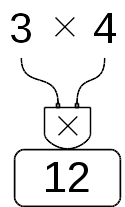
\includegraphics[scale=0.35]{img/op_mol.png}
\end{inaccessibleblock}
\end{minipage}%

Gli operandi della moltiplicazione si chiamano \emph{fattori} e il risultato 
si chiama \emph{prodotto}.

\osservazione Anche per definire la moltiplicazione abbiamo utilizzato 
l'addizione.

\subsubsection{Proprietà}

Dato che per eseguire una moltiplicazione ripeto delle addizioni, 
anche il prodotto di due numeri  naturali qualsiasi è sempre un numero 
naturale. 
Si dice che la moltiplicazione è una \emph{legge di composizione interna}. 

Nei numeri naturali la moltiplicazione presenta le seguenti proprietà:

\begin{itemize*}
 \item \emph{Commutativa}: $a \cdot b = b \cdot a$
 \item \emph{Associativa}: $(a \cdot b) \cdot c = a \cdot (b \cdot c)$
 \item \emph{Elemento neutro} $a \cdot 1 = 1 \cdot a = a$
\end{itemize*}

Un'altra importante proprietà che utilizzeremo spesso anche in seguito è la:

\begin{legge}[Annullamento del Prodotto]
 Il prodotto di due o più numeri naturali si annulla se almeno uno dei fattori 
 è nullo.
\[ a\cdot b=0\Leftrightarrow a=0\text{ oppure }b=0. \]
\end{legge}

Questa legge dice che se il risultato di una moltiplicazione è zero di sicuro
almeno uno dei fattori deve essere zero. Attenzione: questa proprietà non 
vale per tutti gli insiemi numerici in cui è definita la moltiplicazione.

\subsection{Divisione in $\insN$}

Tra i numeri naturali è definita l'operazione di divisione come segue:

\begin{definizione}
Dati due numeri naturali~$m$ e~$n$, con~$n \neq 0$, la divisione associa 
un terzo numero naturale~$q$, se esiste, che moltiplicato per ad~$n$ dà come 
prodotto~$m$.
Si scrive~$n : m = q$.
\end{definizione}

Ad esempio: dividere~12 per~4 significa trovare quante volte il numero~4 è contenuto
nel numero~12.

\begin{minipage}{0.80\textwidth}
 \centering
 $12 : 4 = 3$ perché~$3 \cdot 4 = 12$

% % (c) 2012 Dimitrios Vrettos - d.vrettos@gmail.com

\begin{center}
 \begin{tikzpicture}[decoration={markings,mark=between positions .3 and .5 step 30pt with {\arrowreversed{stealth}}}]
  \begin{scope}[thick,font=\scriptsize]
   \draw[->] (0,0)  - -  (280pt,0) node[above]{$\insN$};
    \foreach \c in {2,3,...,6}{%
     \draw[dotted, color=CornflowerBlue,postaction={decorate}](\c,5pt)--(\c,5pt) arc (180:0:0.5 and 0.5);}
    \foreach \n in {0,1,2,...,9}{%	
     \draw (\n,-3pt) -- (\n,3pt)   node [below=5pt] {$\n$};}
  \end{scope}
 \end{tikzpicture}
\end{center}

\end{minipage}%
\begin{minipage}{0.15\textwidth}
 \centering
\begin{inaccessibleblock}[]
 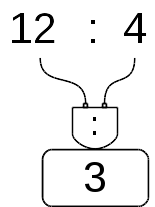
\includegraphics[scale=0.35]{img/op_div.png}
\end{inaccessibleblock}
\end{minipage}%

Il primo operando si chiama \emph{dividendo} e il secondo \emph{divisore}, 
il risultato di dice \emph{quoziente esatto}.

Non sempre si può effettuare la divisione nei numeri naturali ad 
esempio:~$10 : 4 =$ non è un numero naturale.

Se esiste il quoziente esatto tra i numeri $m$ e $n$, si dice che:

\begin{itemize*}
 \item $n$ è \emph{divisore} di~$m$;
 \item $m$ è \emph{divisibile} per~$n$;
 \item $m$ è \emph{multiplo} di~$n$
\end{itemize*}

\begin{exrig}

 \begin{esempio}
$12:3=4$ perché~$4 \times 3 = 12$. Quindi,~12 è divisibile per~3;~3 è un 
divisore di~12;~12 è un multiplo di~3.
 \end{esempio}

 \begin{esempio}
20 è divisibile per~4 perché~$20:4=5$
 \end{esempio}

 \begin{esempio}
7 è divisore di~35 perché~$35:7=5$
 \end{esempio}

 \begin{esempio}
6 è multiplo di~3 perché~$6=2\times~3$
 \end{esempio}

 \begin{esempio}
5 non è multiplo di~3, non esiste alcun numero naturale che moltiplicato 
per~3 dà~5.
 \end{esempio}
\end{exrig}

\osservazione Nella definizione di quoziente abbiamo richiesto che il 
divisore sia diverso da zero. In effetti, se il divisore è~0 non c'è nessun 
numero che moltiplicato per~0 ci possa dare un dividendo diverso da zero.
Per esempio, nella divisione~$5:0$ dobbiamo ottenere un numero che 
moltiplicato per~0 dia~5; ciò non è possibile in quanto qualsiasi numero 
moltiplicato per~0 dà~0.
Invece nella divisione~$0:0$ un qualsiasi numero è adatto come quoziente, 
infatti qualsiasi numero moltiplicato per~0 dà~0 come prodotto.

Nel linguaggio matematico diciamo che una divisione del tipo~$n:0$, 
con~$n\neq~0$, è \emph{impossibile}; mentre la divisione~$0:0$ è 
\emph{indeterminata}.

\osservazione Nella definizione di divisione abbiamo usato l'operazione di 
moltiplicazione che a sua volta usava l'addizione.

\subsubsection{Proprietà}

Dato che non dà sempre un risultato, la divisione non è una 
\emph{legge di composizione interna} ai numeri naturali. 

Non è commutativa né associativa e non ha neppure un elemento neutro.
Possiamo dire che ha solo l'elemento neutro a destra infatti $a : 1 = a$, 
ma in generale non si può fare $1 : a$.

L'unica proprietà interessante della divisione è la proprietà
\begin{itemize*}
 \item \emph{Invariantiva}: 
  $a : b = (a \cdot c) : (b \cdot c) = (a : c) : (b : c) \text{ se } c \neq 0$
\end{itemize*}

Cioè: 
\begin{definizione}
Moltiplicando o dividendo entrambi i termini di una divisione per 
la stessa quantità, \textbf{diversa da zero}, il quoziente non  cambia.
\end{definizione}

\subsection{Proprietà distributiva}

Oltre alle proprietà valide per le singole operazioni, ce n'è una che riguarda 
due operazioni contemporaneamente, è la proprietà \emph{distributiva}.

\subsubsection{Proprietà distributiva della moltiplicazione}

\paragraph{Rispetto all'addizione}
Moltiplicare il risultato dell'addizione di più numeri per un altro numero dà 
lo stesso risultato che moltiplicare ogni addendo per il fattore e addizionare 
i prodotti ottenuti. Questa proprietà vale sia se la somma è a destra sia se è 
a sinistra.

% \begin{flalign*}
%  a\cdot (b+c) &= a\cdot b +a\cdot c & (a+b)\cdot c &=a\cdot c + b\cdot c\\
%  3\cdot(2+4) &=3\cdot 2+3\cdot 4=18 & (2+4)\cdot 3 &=2\cdot 3 + 4\cdot 3=18.
% \end{flalign*}

% alternativa a ``flalign'':

\begin{multicols}{2}
 $a\cdot (b+c) = a\cdot b + a\cdot c$
 
 $(a+b)\cdot c =a\cdot c + b\cdot c$
 
 $3\cdot(2+4) =3\cdot 2 + 3\cdot 4$
 
 $(2+4)\cdot 3 =2\cdot 3 + 4\cdot 3$
\end{multicols}

\paragraph{Rispetto alla sottrazione}
In maniera analoga:

% \begin{flalign*}
%  a\cdot (b-c) &= a\cdot b -a\cdot c & (a-b)\cdot c &=a\cdot c - b\cdot c\\
%  6\cdot(10-4) &=6\cdot 10-6\cdot 4=36 & (10-4)\cdot 6 &=10\cdot 6- 4\cdot 6=36.
% \end{flalign*}

\begin{multicols}{2}
 $a\cdot (b-c) = a\cdot b - a\cdot c$
 
 $(a-b)\cdot c = a\cdot c - b\cdot c$
 
 $6\cdot(10-4) = 6\cdot 10 - 6\cdot 4$
 
 $(2-4)\cdot 6 = 10\cdot 6 - 4\cdot 6$
\end{multicols}

\subsubsection{Proprietà distributiva della divisione}

\paragraph{Rispetto all'addizione}
Solo se le somme sono a sinistra:
\begin{multicols}{2}
 $(a+b+c):d=a:d+b:d+c:d$
 
 $(20+10+5):5=20:5+10:5+5:5=7$
\end{multicols}

Verifichiamo con un esempio che non vale la proprietà distributiva se le somme 
si trovano a destra:~$120:(3+5)$.
Eseguendo prima l'operazione tra parentesi si ottiene 
correttamente~$120:8=15$. Se si prova ad applicare
la proprietà distributiva si ottiene~$120:3+120:5=40+24=64$. 
Il risultato corretto è il \emph{primo}.

\paragraph{Rispetto alla sottrazione}
Solo se la sottrazione è a sinistra:
\begin{multicols}{2}
 $(a-b):c=a:c-b:c$
 
 $(20-10):5=20:5-10:5=4-2=2$
\end{multicols}

Se, però, la sottrazione è a destra:
\[120:(5-3)=120:2=60\neq~120:5-120:3=24-40=\text{ non si può fare.}\]

% \ovalbox{\risolvii \ref{ese:1.8}, \ref{ese:1.9}}

\section{Potenza}
\label{sec:01_potenza}

La \emph{potenza} di un numero naturale è una moltiplicazione che ha tutti i 
fattori uguali.

\begin{definizione}
Dati due numeri naturali~$b$,~$e$, l'operazione di \emph{potenza} 
associa un terzo numero~$p$ che si ottiene moltiplicando~$e$ fattori tutti 
uguali a~$b$:
\begin{inaccessibleblock}[
	$$b^e = \mbox{e volte}{b \cdot b \cdot  \dots  \cdot b} = p$$
	]
$$b^e = \underbrace{b \cdot b \cdot \dots \cdot b}_{\text{e volte}} = p$$
\end{inaccessibleblock}

\end{definizione}

Ma questa definizione è sensata solo nel caso $e$ sia maggiore di~1.
Quindi dobbiamo completarla:

\begin{inaccessibleblock}[
	\begin{definizione}
		$$
		b^e = \begin{cases}
		1 & se \quad e = 0 \text{ e } b\neq 0\\
		b & se \quad e = 1\\
		\mbox{e volte}{b \cdot b \cdot \dots \cdot b} & \mbox{ negli altri casi}
		\end{cases}$$
	\end{definizione}
	]
	\begin{definizione}
		$$
		b^e = \begin{cases}
		1 & se \quad e = 0 \text{ e } b\neq 0\\
		b & se \quad e = 1\\
		\underbrace{b \cdot b \cdot \dots \cdot b}_{e volte} & \text{ negli altri casi}
		\end{cases}$$
	\end{definizione}
\end{inaccessibleblock}


\begin{inaccessibleblock}[]
\begin{minipage}{0.80\textwidth}
 \centering
   % (c) 2012 Dimitrios Vrettos - d.vrettos@gmail.com
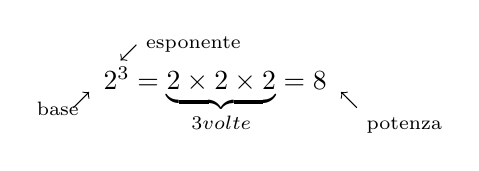
\begin{tikzpicture} 
  \node (esp) at (0,0) {$2^3=\underbrace{2\times 2\times 2}_{3 \text{ volte}} = 8$};
\begin{scope}[font=\scriptsize]
  \draw[<-]  (-1.2,.5)--(-1,.7) node[right] {esponente};
  \draw[->]  (-1.8,-.1)--(-1.6,.1) node[below left=.2] {base};
  \draw[<-]  (1.6,.1)--(1.8,-.1) node[below right] {potenza };
\end{scope}
\end{tikzpicture}

\end{minipage}%
\begin{minipage}{0.15\textwidth}
 \centering
 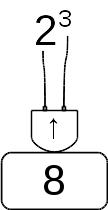
\includegraphics[scale=0.35]{img/op_pot.png}
\end{minipage}%
\end{inaccessibleblock}

Il primo operando si chiama \emph{base}, il secondo \emph{esponente} e il 
risultato si chiama \emph{potenza}.

Da osservare che~$0^0$ non ha significato.

\subsection{Proprietà delle potenze}

\paragraph{I} Il prodotto di più potenze con la stessa base è una 
potenza che ha per base la stessa base e per esponente la somma degli 
esponenti.

\begin{minipage}[h]{.45\textwidth}
\centering
 \begin{empheq}[box=\fbox]{equation*}
 a^n\cdot a^m=a^{n+m}
 \end{empheq}
\end{minipage}\hfil
\begin{minipage}[h]{.45\textwidth}
\centering
\[ 2^5\cdot 2^6=2^{5+6}=2^{11}.\]
\end{minipage}
\vspace{.5cm}

La proprietà segue da questa osservazione:
\begin{inaccessibleblock}[per definizione stessa di potenza]
\[ a^n\cdot a^m = \underbrace{(a\cdot a\cdot\ldots\cdot a)}_{n\text{ volte}}\cdot%
 \underbrace{(a\cdot a\cdot a\cdot\ldots\cdot a)}_{m\text{ volte}}
 =\underbrace{(a\cdot a\cdot a\cdot a\cdot a\cdot\ldots\cdot a\cdot a)}_{n+m\text{ volte}}%
 =a^{n+m}.\]
\end{inaccessibleblock}

\paragraph{II} Il quoziente di due potenze con la stessa base è una 
potenza che ha per base la stessa base e per esponente la differenza degli 
esponenti.

\begin{minipage}[t]{.45\textwidth}
\centering
 \begin{empheq}[box=\fbox]{equation*}
 a^n:a^m=a^{n-m}
 \end{empheq}
\end{minipage}\hfil
\begin{minipage}[t]{.45\textwidth}
\centering
\[4^5:4^3=4^{5-3}=4^2.\]
\end{minipage}
\vspace{.5cm}

La proprietà segue da questa osservazione:
\begin{inaccessibleblock}[per definizione stessa di potenza]
\begin{align}
 a^n: a^m &= \underbrace{(a\cdot a\cdot\ldots\cdot a)}_{n\text{ volte}}:%
 \underbrace{(a\cdot a\cdot a\cdot\ldots\cdot a)}_{m\text{ volte}}\\
 &=\underbrace{(a:a)\cdot(a:a)\cdot\ldots\cdot(a:a)}_{n\text{ volte}}\cdot%
 \underbrace{(a\cdot a\cdot a\cdot\ldots\cdot a)}_{n-m\text{ volte}}\\%
 &=a^{n-m}.
\end{align}
\end{inaccessibleblock}

Il passaggio dalla (1.1) alla (1.2) avviene per la proprietà invariantiva 
della divisione.

\paragraph{III} La potenza di una potenza è una potenza che ha per 
base la stessa base e per esponente il prodotto degli esponenti.

\begin{minipage}[t]{.45\textwidth}
\centering
 \begin{empheq}[box=\fbox]{equation*}
 (a^n)^m=a^{n\cdot m}
 \end{empheq}
\end{minipage}\hfil
\begin{minipage}[t]{.45\textwidth}
\centering
\[(6^2)^5=6^{2\cdot 5}=6^{10}. \]
\end{minipage}
\vspace{.5cm}

La proprietà segue da questa osservazione:

\begin{inaccessibleblock}[definizione stessa di potenza]
\[ (a^n)^m =\overbrace{a^n\cdot a^n\cdot\ldots\cdot a^n}^{m\text{ volte}}%
 =\overbrace{\underbrace{(a\cdot a\cdot\ldots\cdot a)}_{n\text{ volte}}\cdot%
	 \underbrace{(a\cdot a\cdot\ldots\cdot a)}_{n\text{ volte}}\cdot\ldots\cdot%
	 \underbrace{(a\cdot a\cdot\ldots\cdot a)}_{n\text{ volte}}}^{m\text{ volte}}%
	 =a^{n\cdot m}.\]
\end{inaccessibleblock}

\paragraph{IV} Il prodotto di più potenze con lo stesso esponente è
una potenza che ha per base il prodotto delle basi e per esponente lo stesso
esponente.

\begin{minipage}[t]{.45\textwidth}
\centering
 \begin{empheq}[box=\fbox]{equation*}
 (a\cdot b)^n=a^n\cdot b^n
 \end{empheq}
\end{minipage}\hfil
\begin{minipage}[t]{.45\textwidth}
\centering
\[(2\cdot 5)^8=2^8\cdot 5^8. \]
\end{minipage}
\vspace{.5cm}

La proprietà segue da questa osservazione:
\begin{inaccessibleblock}[definizione stessa di potenza]
\[(a\cdot b)^n=\underbrace{(a\cdot b)\cdot(a\cdot b)\cdot\ldots\cdot(a\cdot b)}_{n\text{ volte}}%
	 =\underbrace{(a\cdot a\cdot\ldots\cdot a)}_{n\text{ volte}}\cdot%
	 \underbrace{(b\cdot b\cdot\ldots\cdot b)}_{n\text{ volte}}%
	 =a^n\cdot b^n.\]
\end{inaccessibleblock}

\paragraph{V} Il quoziente di due potenze con lo stesso esponente è
una potenza che ha per base il quoziente delle basi e per esponente lo stesso
esponente.

\begin{minipage}[t]{.45\textwidth}
\centering
 \begin{empheq}[box=\fbox]{equation*}
 (a:b)^n=a^n:b^n
 \end{empheq}
\end{minipage}\hfil
\begin{minipage}[t]{.45\textwidth}
\centering
\[(4:2)^8=4^8:2^8. \]
\end{minipage}
\vspace{.5cm}

Le definizioni dei casi particolari di potenze si giustificano nel seguente 
modo:

\begin{align*}
 &a^0=a^{5-5}=a^5:a^5=1,\\
 &a^1=a^{5-4}=a^5:a^4=a.
\end{align*}

Alla potenza~$0^0$ non si assegna alcun valore perché applicando la 
definizione di~$a^0$ si dovrebbe ottenere~1;
applicando la definizione~$0^a$ si dovrebbe ottenere~0, 
ma non è accettabile che il risultato dipenda da una scelta arbitraria della 
regola da usare.

% \ovalbox{\risolvii \ref{ese:1.10}, \ref{ese:1.11}, \ref{ese:1.12}, 
%  \ref{ese:1.13}, \ref{ese:1.14}, \ref{ese:1.15}}\vspazio

\section{Espressioni numeriche}
\label{sec:01_espressioni}

Spesso in matematica abbiamo a che fare con più operazioni combinate assieme.
In questo caso parliamo di espressioni:

\begin{definizione}
 Un'espressione aritmetica è una successione di operazioni.
\end{definizione}

Nel linguaggio comune alcune frasi possono risultare ambigue. Per esempio
<<Luca ha detto Mario è stato promosso>> può avere due significati diversi
a seconda di come si inserisce la punteggiatura:
scrivendo <<Luca, ha detto Mario, è stato promosso>> significa che è stato 
promosso Luca;
scrivendo <<Luca ha detto: Mario è stato promosso>> significa che è stato 
promosso Mario.

Anche nella matematica, quando abbiamo più operazioni da eseguire, dobbiamo 
chiarire l'ordine con cui si devono eseguire le operazioni. 
Per esempio, l'espressione~$7+5\cdot2$ può valere~24 oppure~14, infatti:
eseguendo le operazioni da sinistra a destra (associatività a sinistra) 
otteniamo~24 (vedi figura~\ref{fig:op_prec1}), 
mentre eseguendo prima la moltiplicazione (precedenza algebrica) otteniamo~17
(vedi figura~\ref{fig:op_prec2}).
 
\begin{inaccessibleblock}[]
\begin{figure}[h]
 \centering
 \begin{minipage}[t]{.40\textwidth}
  \centering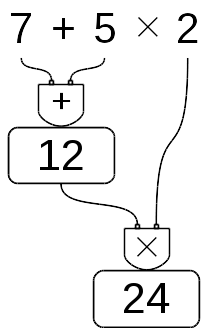
\includegraphics[scale=0.35]{img/op_prec1.png}
  \caption{Da sinistra a destra.}\label{fig:op_prec1}
 \end{minipage}\hfil
 \begin{minipage}[t]{.50\textwidth}
  \centering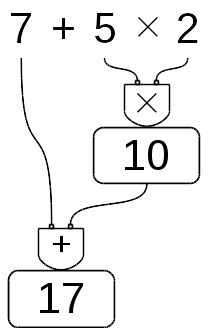
\includegraphics[scale=0.35]{img/op_prec2.png}
  \caption{Precedenza alle moltiplicazioni.}\label{fig:op_prec2}
 \end{minipage}
\end{figure}
\end{inaccessibleblock}

\osservazione Alcune calcolatrici, quelle ``aritmetiche'' svolgono le 
operazioni man mano che sono inserite, si dice che applicano 
\emph{l'associatività a sinistra}. Altre, le calcolatrici ``scientifiche'' 
seguono le regole dell'algebra. Esegui la seguente sequenza di operazioni 
sulla tua calcolatrice 
(le barre verticali separano i diversi tasti da premere):

\begin{verbatim}
 |7|+|5|×|2|=|
\end{verbatim} 

Osserva il risultato e confrontalo poi con quello ottenuto dai tuoi compagni.
Diverse calcolatrici possono fornire risultati diversi.
Per eliminare queste ambiguità sono state fissate le tre regole della 
precedenza algebrica:

\begin{enumerate}
 \item prima si svolgono le espressioni nelle parentesi più interne; 
 \item in una espressione senza parentesi si svolgono prima le potenze, 
  poi moltiplicazioni e divisioni, poi addizioni e sottrazioni;
 \item le operazioni con la stessa precedenza si svolgono da sinistra verso 
  destra.
\end{enumerate}

\subsection{Soluzione con grafo ad albero}

Risolviamo le espressioni con i numeri naturali usando grafi ad albero;
gli operandi sono le foglie dell'albero, il risultato è la radice. 
Costruiamo il grafo tenendo conto delle seguenti indicazioni:

\begin{procedura}
 Per risolvere un'espressione usando un grafo:
\begin{enumerate*}
 \item in ogni nodo viene riportata l'operazione eseguita e il risultato;
 \item costruiamo l'albero disegnando ogni nodo esattamente sotto
  l'operazione corrispondente;
 \item disegniamo le parentesi attorno al nodo che contiene il
  risultato di tutta un'espressione racchiusa tra parentesi.
\end{enumerate*}
\end{procedura}

Vediamo, con un esempio, come fare.
% \newpage

\begin{exrig}
 \begin{esempio}
  $49 - [2^4 \times (14 : 7) + 10]=$
  
\begin{inaccessibleblock}[Descrizione immagine: TODO]
 \begin{center}
  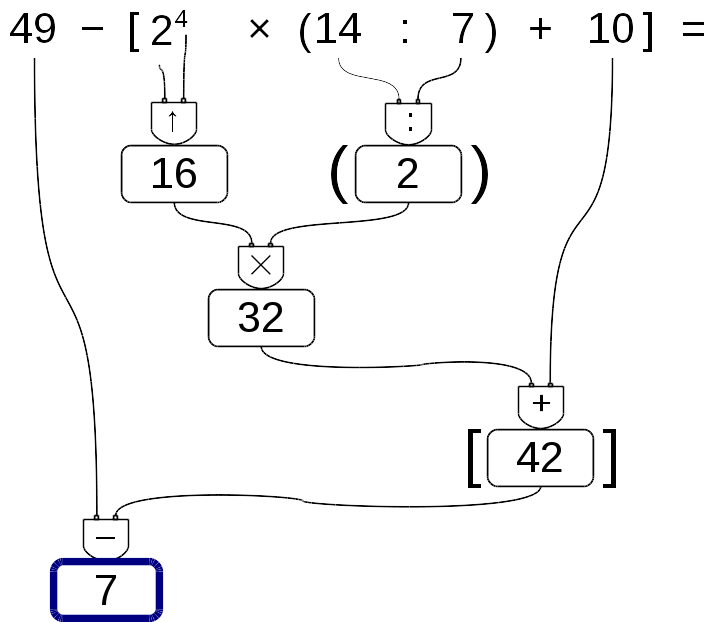
\includegraphics[scale=0.35]{img/op_espr.png}
 \end{center}
\end{inaccessibleblock}
 \end{esempio}

 \begin{esempio}
  $8^9 \times 8^5 : (8^3)^4 : [4^{12} : (4^2)^5] + 27^2 : 9^2 =$
  
  Se per risolvere un'espressione dobbiamo utilizzare le proprietà delle 
  potenze, al posto del simbolo di operazione scriveremo le 
  sigle~``p1'',~``p2'',~\dots per indicare l'uso della prima, seconda,~\dots
  proprietà.
  
\begin{inaccessibleblock}[]
 \begin{center}
  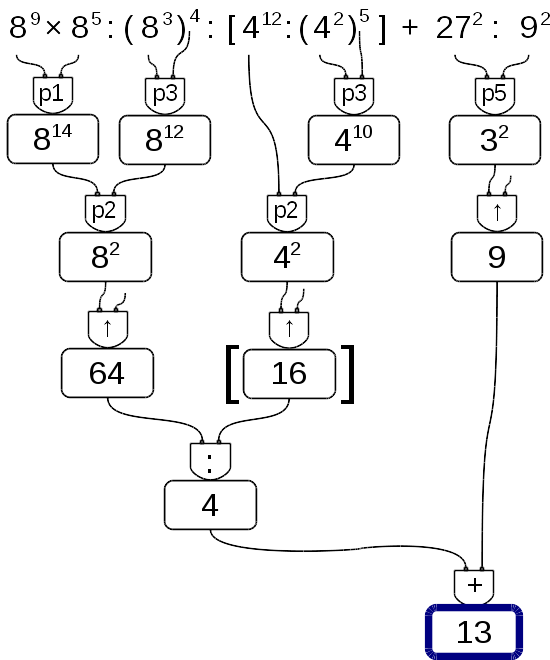
\includegraphics[scale=0.35]{img/op_espr_pot.png}
 \end{center}
\end{inaccessibleblock}
 \end{esempio}
\end{exrig}

\subsection{Metodo sequenziale}

In alcuni casi può non essere comodo, o praticabile, l'uso di un grafo ad 
albero per risolvere espressioni vediamo allora il metodo sequenziale che
prevede di copiare tutta o in parte l'espressione rendendola via via più 
semplice. Possiamo applicare le seguenti indicazioni:

\begin{procedura}
 Per risolvere un'espressione in modo sequenziale:
\begin{enumerate*}
 \item scorriamo tutta l'espressione da sinistra a destra 
 e sottolineiamo tutte le operazioni che si possono eseguire;
 \item riscriviamo l'espressione sostituendo alle operazioni sottolineate,
 nel passo precedente, i loro risultati.
\end{enumerate*}
\end{procedura}

Partiamo da una nuova espressione:

$2 + 6 \times 2 \div 
 \left[ \left(4 -2 \right) \times 3^{2} - 3 \times 5 \right] +
 \left( 5^{2} + 2^{3} \right) \div 3 =$
 
Scorrendo l'espressione vediamo che l'operazione~$2 + 6$ è seguita da una 
moltiplicazione; poiché la moltiplicazione ha la precedenza sull'addizione,
non possiamo eseguire~$2 + 6$. La prossima espressione che incontriamo 
è~$6 \times 2$ dato che è seguita da una divisione possiamo eseguirla e 
quindi la sottolineiamo. Procediamo così sottolineando tutte le operazioni
che possiamo eseguire, a questo punto della soluzione, rispettando le
precedenze algebriche:

$2 + 
 \underline{6 \times 2} \div \left[ \underline{\left(4 -2 \right)} 
   \times \underline{3^{2}} - 
   \underline{3 \times 5} \right] +
 \left( \underline{5^{2}} + \underline{2^{3}} \right) \div 3 =$

Ora ricopiamo l'espressione sostituendo al posto delle operazioni sottolineate
il loro risultato:

$= 2 + 
 12 \div \left[ 2 \times 9 - 15 \right| +
 \left( 25 + 8 \right) \div 3 =$

Otteniamo così un'espressione a cui applicare nuovamente i due passi 
precedenti fino ad averla ridotta ad un numero.

Sottolineo:

$= 2 + 
 12 \div \left[ \underline{2 \times 9} - 15 \right| +
 \underline{\left( 25 + 8 \right)} \div 3 =$

Eseguo:

$= 2 + 12 \div \left[ 18 - 15 \right| +
 33 \div 3 =$

Sottolineo:

$= 2 + 
 12 \div \underline{\left[ 18 - 15 \right|} +
 \underline{33 \div 3} =$

Eseguo:

$= 2 + 
 12 \div 3 +
 11 =$
 
Sottolineo:
 
$= 2 + 
 \underline{12 \div 3} +
 11 =$

Eseguo:

$= 2 + 
 4 +
 11 =$

Sottolineo:

$= \underline{2 +  4} + 11 =$

Eseguo:

$= 6 + 11 = 17$

Nell'ultimo passaggio, essendo rimasta una sola operazione, è inutile 
sottolinearla. Avremmo anche potuto risolvere con un passaggio in meno
calcolando assieme le due addizioni:

$= 2 + 4 + 11 = 17$

\section{Espressioni con un buco}
\label{sec:01_espressioni_buco}

A volte potrà succedere che, nell'espressione, manchi un numero.
Conoscendo il risultato possiamo trovare il numero mancante.

\subsection{Soluzione con grafo ad albero}

\begin{procedura}
 Per trovare l'operando mancante usando il grafo ad albero:
\begin{enumerate*}
 \item costruiamo il grafo risolutivo senza eseguire operazioni;
 \item eseguiamo tutte le operazioni possibili;
 \item scriviamo il risultato nella radice;
 \item con un colore diverso completiamo il grafo risalendo fino al numero 
  mancante.
\end{enumerate*}
\end{procedura}

Vediamo, con qualche esempio, come fare.

\begin{exrig}
\begin{esempio}
  Nella seguente espressione manca un esponente:
  
  $[4 \times 5 + 16 : 2 - (13 - 2^{\dots}) \times 2] : 2 = 9$
 
  Costruiamo il grafo risolutivo vuoto, eseguiamo tutte le operazioni 
  possibili. Ora, usando un colore diverso, scriviamo nella radice il 
  risultato dell'espressione. 
  
\begin{inaccessibleblock}[]
 \begin{center}
  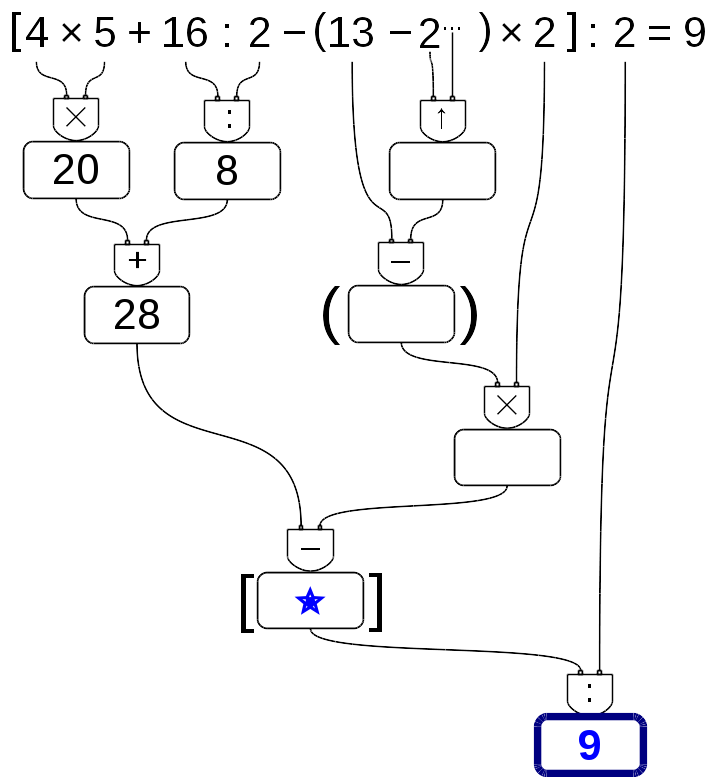
\includegraphics[scale=0.35]{img/op_buco1.png}
 \end{center}
\end{inaccessibleblock}
  
  Ora poniamo attenzione al nodo vuoto che precede il risultato, 
  il nodo contrassegnato dalla stella.
  Dobbiamo trovare il numero che diviso per~2 dia come risultato~9. È facile:
  il numero cercato è~18. Scriviamo allora~18 in questo nodo e poniamo
  l'attenzione a quello che lo precede.
  
\begin{inaccessibleblock}[]
 \begin{center}
  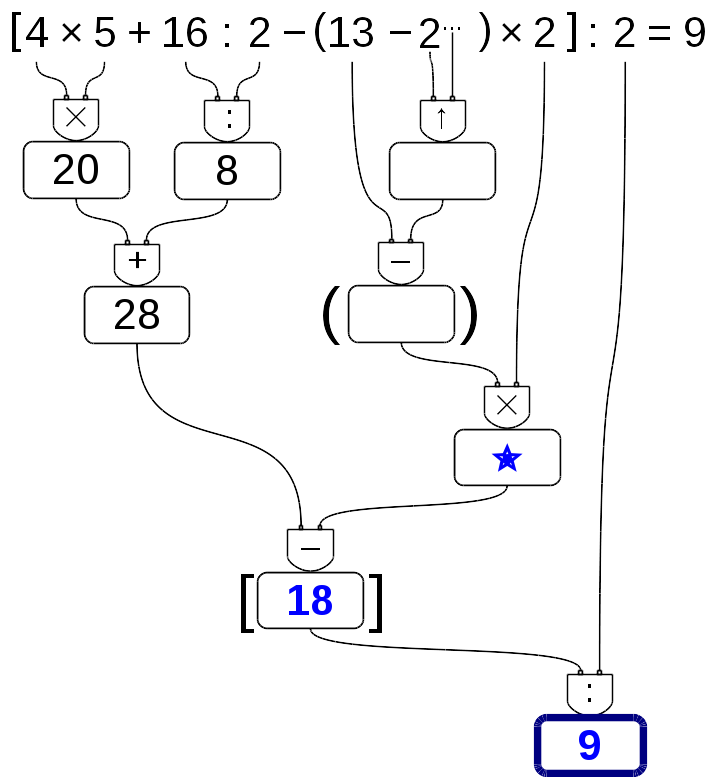
\includegraphics[scale=0.35]{img/op_buco2.png}
 \end{center}
\end{inaccessibleblock}
 
  Ora dobbiamo trovare quel numero che tolto da~28 dia come risultato~18. 
  Anche questo è facile da trovare: è~10. Lo scriviamo e ci spostiamo
  sul nodo precedente. Procedendo in questo modo possiamo risalire fino
  al dato mancante:
  
\begin{inaccessibleblock}[]
 \begin{center}
  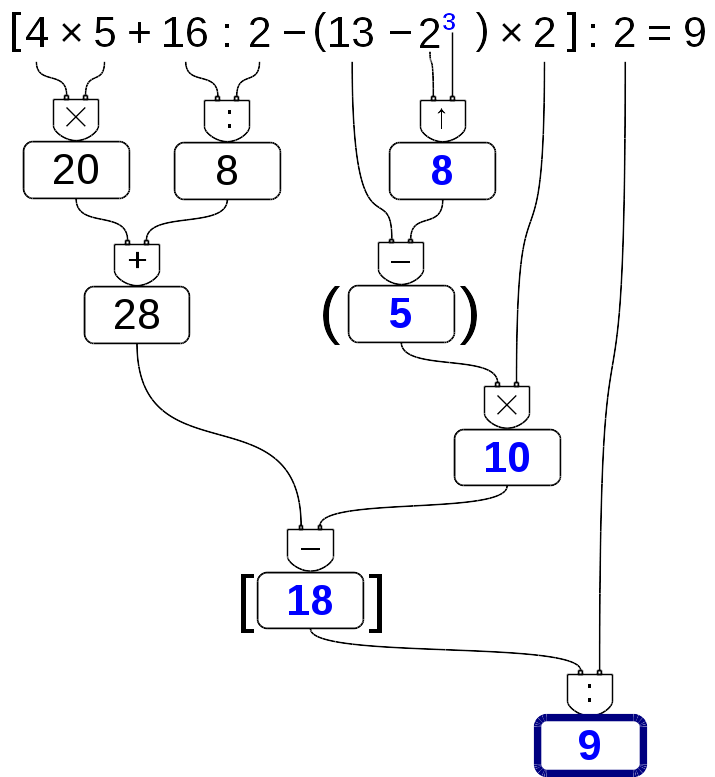
\includegraphics[scale=0.35]{img/op_buco3.png}
 \end{center}
\end{inaccessibleblock}
 \end{esempio}

 \begin{esempio}
  Se c'è un ``buco'' in una espressione da risolvere con le proprietà delle 
  potenze, si procede allo stesso modo:
  
  $(3^4)^3 \times 3^{\dots} : (3^3)^5 -2^3 \times 2 \times (20 -3 \times 5 ) = 1$
 
  Costruiamo il grafo risolutivo eseguendo tutte le operazioni possibili. 
  Rimangono vuoti tutti i nodi che collegano la radice all'elemento
  mancante. Usando un colore diverso, a partire dalla radice, completiamo
  il grafo. Scriviamo nella radice il risultato dell'espressione, e poniamo 
  attenzione 
  al nodo vuoto che lo precede.
  
\begin{inaccessibleblock}[]
 \begin{center}
  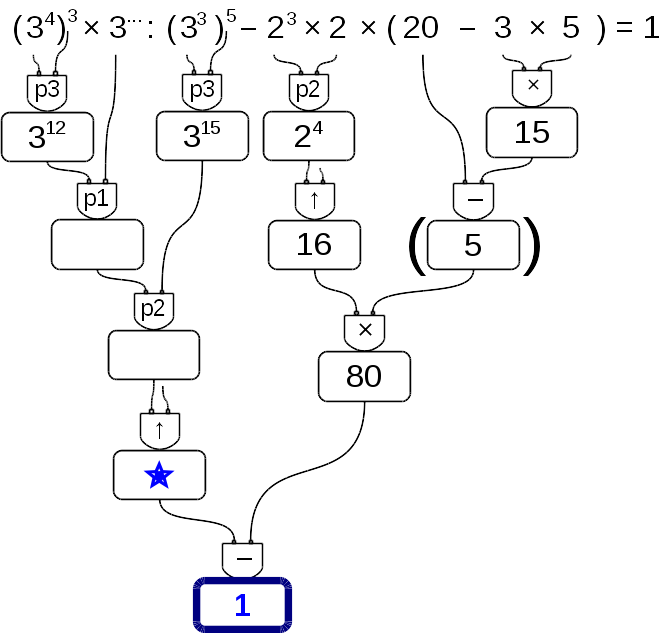
\includegraphics[scale=0.35]{img/op_buco4.png}
 \end{center}
\end{inaccessibleblock}

È facile individuare i valori mancanti:
  
\begin{itemize*}
 \item questo numero meno ottanta deve dare come risultato uno: il numero 
  cercato è~81; 
 \item nel nodo precedente: qui ci va una potenza che deve dare come 
  risultato~81, potrebbe essere~$9^2$ o~$3^4$, ma dato che sopra posso usare 
  le proprietà delle potenze con base~3, conviene usare~$3^4$; 
 \item nel nodo precedente: questo esponente meno quindici deve dare come 
  risultato quattro, l'esponente qui deve essere 19;
 \item e infine: dodici sommato a questo esponente deve dare come risultato 
  diciannove: il valore mancante è quindi:~7.
\end{itemize*}

 \end{esempio}

\begin{esempio}
  Prova a risolvere questa:
  
  $(3^4)^3 \times 3^{\dots} : (3^3)^5 -2^3 \times 2 \times (20 -3 \times 5 ) = 1$
 
  Costruiamo il grafo risolutivo eseguendo tutte le operazioni possibili. 
  Rimangono vuoti tutti i nodi che collegano la radice all'elemento
  mancante. Usando un colore diverso, a partire dalla radice, completiamo
  il grafo. Scriviamo nella radice il risultato dell'espressione, e poniamo attenzione 
  al nodo vuoto che lo precede.
  
\begin{inaccessibleblock}[]
 \begin{center}
  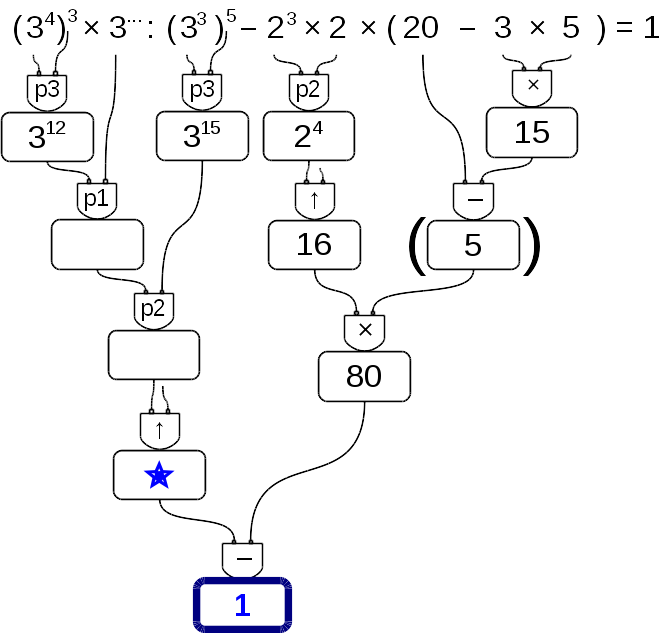
\includegraphics[scale=0.35]{img/op_buco4.png}
 \end{center}
\end{inaccessibleblock}

È facile individuare i valori mancanti:
  
\begin{itemize*}
 \item questo numero meno ottanta deve dare come risultato uno: il numero 
  cercato è~81; 
 \item nel nodo precedente: qui ci va una potenza che deve dare come 
  risultato~81, potrebbe essere~$9^2$ o~$3^4$, ma dato che sopra posso usare 
  le proprietà delle potenze con base~3, conviene usare~$3^4$; 
 \item nel nodo precedente: questo esponente meno quindici deve dare come 
  risultato quattro, l'esponente qui deve essere 19;
 \item e infine: dodici sommato a questo esponente deve dare come risultato 
  diciannove: il valore mancante è quindi:~7.
\end{itemize*}

 \end{esempio}

\end{exrig}

\subsection{Soluzione sequenziale}

\begin{procedura}
 Per trovare l'operando mancante usando il metodo sequenziale:
\begin{enumerate*}
 \item risolviamo l'espressione lasciando il buco ogni volta che 
  dobbiamo eseguire un'operazione tra un numero e un buco;
 \item scriviamo il risultato dopo l'ultima operazione;
 \item con un colore diverso risaliamo dalla soluzione al dato mancante
  chiudendo man mano tutti i buchi.
\end{enumerate*}
\end{procedura}

Vediamo, con qualche esempio, come fare.

\begin{exrig}
  \begin{esempio}
  $\left[ 4 \times 5 + 16 \div 2 -
   \left(13 - 2^{\dots} \right) \times 2 \right] \div 2 = 9$
  
  Come al solito iniziamo sottolineando tutte le operazioni che dobbiamo 
  eseguire a questo punto:
  
  $\left[ \underline{4 \times 5} + \underline{16 \div 2} -
   \left(13 - \underline{2^{\dots}} \right) \times 2 \right] \div 2 = 9$
  
  Ora, sostituiamo tutte le operazioni sottolineate con il loro risultato, 
  tutte tranne l'operazione che contiene il buco: il suo risultato sarà un 
  buco:
  
  $\left[ 20 + 8 -
   \left(13 - {\dots} \right) \times 2 \right] \div 2 = 9$
   
  procediamo sottolineando e eseguendo:
  
  $\left[ \underline{20 + 8} -
   \underline{\left(13 - {\dots} \right)} \times 2 \right] \div 2 = 9$
  
  $\left[ 28 - \underline{{\dots} \times 2} \right] \div 2 = 9$
  
  $\underline{\left[ 28 - {\dots} \right]} \div 2 = 9$
  
  $\underline{{\dots} \div 2} = 9$
  
  Ora possiamo risalire: cambiamo colore e\dots
  
  \begin{itemize*}
   \item il numero che diviso per~2 dà~9 è~18;
   \item il numero che tolto da~20 dà~18 +~10;
   \item il numero che moltiplicato per~2 dà~10 è~5;
   \item \dots
  \end{itemize*}

 E così arriviamo a scoprire che il dato mancante è: \dots.
 
 \end{esempio}

 \begin{esempio}

 Possiamo anche risolvere espressioni con il buco dove bisogna
 applicare le proprietà delle potenze:
 
 $\left(3^4 \right)^3 \cdot 3^{\dots} \div \left(3^3 \right)^5 -
  2^{3} \cdot 2 \cdot \left( 20 - 3 \cdot 5 \right) = 1$

 $\underline{\left(3^4 \right)^3} \cdot 
  3^{\dots} \div \underline{\left(3^3 \right)^5} -
  \underline{2^{3} \cdot 2} \cdot 
  \left( 20 - \underline{3 \cdot 5} \right) =$

 $\underline{3^{12} \cdot 3^{\dots}} \div 3^{15} -
  \underline{2^{4}} \cdot \underline{\left( 20 - 15 \right)} =$

  $\underline{3^{\dots}} \div 3^{15} -
  \underline{16 \cdot 5} =$

  $\underline{3^{\dots}} - 80 =$

  $\underline{{\dots} - 80} =$
  
  $1$

  La risalita non dovrebbe creare problemi.
  
 \end{esempio}
\end{exrig}

\section{Divisibilità e numeri primi}
\label{sec:01_divsibilita}

Come hai potuto notare dagli esercizi precedenti la divisione tra due numeri 
naturali non è sempre possibile.

\osservazione In~$\insN$ la divisione tra due numeri,~$m$ e~$n$, è possibile 
solo se~$m$ è multiplo di~$n$.

Con i numeri naturali però è sempre possibile eseguire la divisione con il 
resto. La \emph{divisione con resto} è un'operazione che dà due risultati:
il \emph{quoziente} e il \emph{resto}.

\begin{definizione}
 Dati due numeri naturali~$m$ e~$n$, con~$n\neq~0$, 
 possiamo sempre trovare due numeri $q$ e $r$ con $0 \leqslant r < n$ 
 tali che: 
 $$m = n \cdot q + r$$ 
 $q$ si dice \emph{quoziente} e $r$ si dice \emph{resto} della divisione.
\end{definizione}

\begin{exrig}
 \begin{esempio}
 Nella divisione con resto tra~25 e~7 si ha quoziente~3 
 (infatti~$7\times~3=21$,
 mentre~$7\times~4=28$ supera il dividendo) e resto~4 
 (infatti~$3 \times 7 + 4 = 25$).

\begin{inaccessibleblock}[Algoritmo della divisione tra 25 e 7]
 % (c) 2012 Dimitrios Vrettos - d.vrettos@gmail.com

\begin{center}
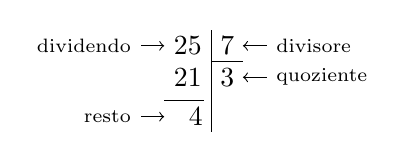
\begin{tikzpicture}

\draw[-](0,.4)--(0,-.9); % verticale
\draw[-](0,0)--(.4,0) ; %orizzontale
\draw (-.1,-.5) -- (-.6,-.5); % resto

\node (a) at (.2,.2) {7};
\node (b) at (.2,-.2) {3};
\node (c) at (-.3,.2) {25};
\node (d) at (-.3,-.2) {21};
\node (e) at (-.2,-.7){4};

\begin{scope}[font=\scriptsize]
  \draw  [<-] (.4,.2)--(.7,.2) node[right] {divisore};
  \draw  [<-] (.4,-.2)--(.7,-.2) node[right] {quoziente};
  \draw  [<-] (-.6,.2)--(-.9,.2) node[left] {dividendo};
  \draw  [<-] (-.6,-.7)--(-.9,-.7) node[left] {resto};
\end{scope}

\end{tikzpicture}

\end{center}

\end{inaccessibleblock}
 \end{esempio}

 \begin{esempio}
 Alcune semplici divisioni con il resto:
 
\begin{multicols}{2}
$0:2 = \text{ quoziente=0 e resto=0}$

$3:0 = \text{ non si può fare}$

$1:2 = \text{ quoziente=0 e resto=1}$

$7:2 = \text{ quoziente=3 e resto=1}$
\end{multicols}

 \end{esempio}
\end{exrig}

Un'operazione che dà due risultati a volte è scomoda quindi i matematici 
hanno ricavato, dalla divisione con resto, due nuove operazioni: 
la \emph{divisione intera} e il \emph{modulo}.

\begin{definizione}
 Dati due numeri naturali~$n$ e~$m$, con~$m\neq~0$, la 
 \emph{divisione intera}~$n\divint m$ è l'operazione che dà il più grande 
 numero naturale~$q$ (il quoziente) per il quale si ha
$$q\times m\le n$$
\end{definizione}

\newpage

\begin{exrig}
 \begin{esempio}
 Alcune semplici divisioni intere:
 
\begin{multicols}{2}
$0 \divint 5=0$

$9 \divint 2=4$

$3\divint 5=0$

$3\divint~0=\text{ non si può fare.}$
\end{multicols}

 \end{esempio}
\end{exrig}

\begin{definizione}
 Dati due numeri naturali~$n$ e~$m$, con~$m\neq~0$, l'operazione che 
 restituisce il resto della divisione intera tra~$n$ e~$m$ si chiama 
 \emph{modulo} di~$n$ rispetto a~$m$ e viene indicata con~$n\bmod{m}$.
\end{definizione}

\begin{exrig}
 \begin{esempio}
 Alcuni esempi di modulo:
 
\begin{multicols}{2}
$3 \bmod 0= \text{ non si può fare}$

$0 \bmod 5= 0$

$9 \bmod 5 = 4$

$10 \bmod 5 = 0$

$3 \bmod 5 = 3$

$11 \bmod 5 = 1$.
\end{multicols}

 \end{esempio}
\end{exrig}

% \ovalbox{\risolvii \ref{ese:1.2}, \ref{ese:1.3}, \ref{ese:1.4}, 
%  \ref{ese:1.5}, \ref{ese:1.6}}\vspazio

Ripassiamo l'algoritmo della divisione intera per numeri a più cifre; questo 
algoritmo risulterà particolarmente utile nel seguito.

\vspace{-6pt}
\begin{center}
\begin{inaccessibleblock}[
Algoritmi della divisione tra 327 e 23, 1329 e 107, 12594 e 171]
 % (c) 2012 Dimitrios Vrettos - d.vrettos@gmail.com

\begin{tikzpicture}[node distance=-25ex]
	\begin{scope}[font=\ttfamily]
 	\matrix (divisione) [matrix of nodes]
 	{%
 		&	3 & 2	&	7	&	2	&	3 &[.8cm] & 1 & 3 & 2 & 9 & 1 & 0 & 7 &[.8cm]   & 1 & 2	& 5	& 9 & 4 & 3 & 1 & 7 & 1\\
 	 |[gray]| -	& 2 & 3 &  	& |[blue]|1 & |[blue]|4 &  			|[gray]| -& 1 & 0 & 7 &  	  & |[blue]|1 & |[blue]|2	  &  	  & |[gray]|- & 1 & 1 	& 9 & 7 &  	&  	& |[blue]|7 & |[blue]|3 & |[blue]|6\\
 	   	&   	& 9 & 7 &  	&  	& 			  &	  & 2 & 5 & 9 &  	  &		  &  	 &  &     &  & 6 & 2 & 4 &  &  &  & \\
       &|[gray]|-  & 9 & 2 &  &  &  &|[gray]|  - & 2 & 1 & 4 &  &  &  &  &     &|[gray]| - & 5 & 1 & 3 &  &  &  & \\
      &  &  & |[red]|5 &  &  &  &   &  & |[red]|4 & |[red]|5 &  &  &  &  &     &  & 1 & 1 & 1 & 3 &  &  & \\
	 &  &  &  &  &  &  &   &  &  &  &  &  &  &  &     & |[gray]|- & 1 & 0 & 2 & 6 &  &  & \\
	&  &  &  &  &  &  &   &  &  &  &  &  &  &  &     &  &  &  & |[red]|8 & |[red]|	7 &  &  & \\
 	};
	\end{scope}
	% Prima divisione
	\draw(divisione-1-5.north west)--(divisione-1-5.south west);
	\draw(divisione-1-5.south west)--(divisione-1-6.south east);
	\draw(divisione-2-2.south west)--(divisione-2-3.south east);
	\draw(divisione-4-3.south west)--(divisione-4-4.south east);
	% Seconda divisione
	\draw (divisione-1-12.north west) -- (divisione-1-12.south west);
	\draw (divisione-1-12.south west) -- (divisione-1-14.south east);
	\draw(divisione-2-8.south west)--(divisione-2-10.south east);
	\draw (divisione-4-9.south west) -- (divisione-4-11.south east);
	% Terza divisione
	\draw (divisione-1-22.north west) -- (divisione-1-22.south west);
	\draw (divisione-1-22.south west) -- (divisione-1-24.south east);
	\draw (divisione-2-16.south west) -- (divisione-2-19.south east);
	\draw (divisione-4-18.south west) -- (divisione-4-20.south east);
	\draw (divisione-6-18.south west) -- (divisione-6-21.south east);
	% Frecce
	\draw[densely dotted,->] (divisione-1-4) -- (divisione-3-4);
	\draw[densely dotted,->] (divisione-1-11) -- (divisione-3-11);
	\draw[densely dotted,->] (divisione-1-20) -- (divisione-3-20);
	\draw[densely dotted,->] (divisione-1-21) -- (divisione-5-21);
	% Didascalie
	\node (a) [above=of divisione-1-5.north west] {(a)};
	\node (b) [above=of divisione-1-12.north west] {(b)};
	\node (c) [above=of divisione-1-22.north west] {(c)};
\end{tikzpicture}

\end{inaccessibleblock}
\end{center}
\vspace{-12pt}

\begin{enumeratea}
 \item $327:23=$ quoziente~14 e resto~5;
 \item $1329:107=$quoziente~12 e resto~45;
 \item $125943:171=$ quoziente~736 e resto~87.
\end{enumeratea}

\subsection{Divisori, numeri primi, numeri composti}

Precisiamo il significato di \emph{divisore} con la seguente definizione:

\begin{definizione}
 Il numero $n$ si dice divisore di $m$ se, nella divisione intera, 
 $m : n$ dà come resto~0.
\end{definizione}

Prima di proseguire, disegna nel quaderno la seguente tabella e completala.  
Nella prima colonna scrivi i numeri fino al~50, nella seconda scrivi tutti 
i divisori di quel numero ordinati dal minore al maggiore, nella terza 
scrivi quanti sono i divisori.

\begin{table}[h]
\centering
\caption{Divisori dei primi numeri naturali}
\begin{tabular}{|r|p{6cm}|c|}
\hline
\textsf{\relax 
numero
} & \textsf{\relax 
          divisori          
} & \textsf{\relax 
numero di divisori
}\\
\hline
0 & tutti i numeri naturali & $\infty$\\
\hline
1 & 1 & 1\\
\hline
2 & 1, 2 & 2\\
\hline
3 & 1, 3 & 2\\
\hline
4 & 1, 2, 4 & 3\\
\hline
5 & 1, 5 & 2\\
\hline
6 &  & \\
\hline
7 &  & \\
\hline
8 &  & \\
\hline
9 &  & \\
\hline
10 &  & \\
\hline
11 &  & \\
\hline
\dots &  & \\
\hline
\end{tabular}
\end{table}

\begin{enumeratea}
 \item Quale sarà il prossimo numero con un numero dispari 
  di divisori? (\emph{facile})
 \item Quale sarà il prossimo numero con esattamente~2
  divisori? (\emph{impossibile?})
\end{enumeratea}

Guardando la tabella dei divisori si può osservare che ogni numero è 
divisibile per~1 e per se stesso. Poi può avere altri divisori, questi
altri divisori si chiamano divisori propri.

\begin{definizione}
 Chiamiamo \emph{divisore proprio} di un numero un divisore diverso dal 
 numero stesso e dall'unità.
\end{definizione}

Per quanto riguarda il numero dei divisori possiamo anche osservare che 
due numeri sono particolari:

\begin{itemize*}
 \item \emph{zero} è divisibile per ogni numero naturale perché quando 
  dividiamo~0 per un qualunque numero otteniamo come resto~0.
 \item \emph{uno} ha un solo divisore.
\end{itemize*}

Dopo queste osservazioni possiamo dare le seguenti definizioni:

\begin{definizione}
 Un numero~$p>1$ si dice \emph{primo} se ha esattamente due divisori. 
\end{definizione}

\begin{definizione}
 Un numero~$p>1$ si dice \emph{quadrato} se ha un numero dispari di divisori. 
\end{definizione}

\begin{definizione}
 Un numero~$p>1$ si dice \emph{composto} se ha più di due, ma non infiniti, 
 divisori. 
\end{definizione}

Nella tabella dei divisori evidenzia i numeri primi e con un colore diverso i 
numeri quadrati.

\osservazione~2 è l'unico numero primo pari.

% \ovalbox{\risolvi \ref{ese:1.16}}\vspazio

Ma quanti sono i numeri primi? La risposta a questa domanda venne data da 
Euclide con il seguente teorema che porta il suo nome:

\begin{teorema}[di Euclide]
I numeri primi sono infiniti.
\end{teorema}

Euclide ci ha fatto vedere come sia possibile costruire numeri primi comunque 
grandi. Dato un numero primo, è sempre possibile costruirne uno più grande.

% \vspazio\ovalbox{\risolvi \ref{ese:1.17}}

\osservazione Un numero è primo quando non è divisibile per nessun numero 
primo compreso tra~2 e la radice quadrata del numero.

\subsubsection{Criteri di divisibilità}
\label{sec:01_divisibilita}

Per vedere se un numero divide un altro \emph{basta} eseguire la 
divisione e osservare se si ottiene un resto uguale a zero. 
Ma questo non sempre è comodo da fare, i matematici hanno scoperto dei
trucchi per capire se un numero divide un altro senza dover eseguire 
la divisione: sono i \emph{criteri di divisibilità}. 
Di seguito sono riportati i criteri relativi ai primi numeri naturali.

\paragraph{Divisibilità per~0} Nessun numero è divisibile per~0.

\paragraph{Divisibilità per~1} Tutti i numeri sono divisibili per~1.

\paragraph{Divisibilità per~2}~0,~2,~4,~6,~8 sono divisibili per~2 
e un numero è divisibile per~2 se e solo se il numero formato dalla sua 
ultima cifra è divisibile per~2.

\paragraph{Divisibilità per~3}~0,~3,~6,~9 sono divisibili per~3,
e un numero è divisibile per~3 se e solo se la somma delle sue cifre è un 
numero è divisibile per~3.

\paragraph{Divisibilità per~4}~0,~4,~8,~12,~16,~20,~24,~28,~32,~36 \dots sono 
divisibili per~4 
e un numero è divisibile per~4 se e solo se il numero formato dalle sue 
ultime~2 cifre, è divisibile per~4.

\paragraph{Divisibilità per~5}~0,~5 sono divisibili per~5 
e un numero è divisibile per~5 se e solo se il numero formato dalla sua 
ultima cifra è divisibile per~5.

\paragraph{Divisibilità per~6} Un numero è divisibile per~6 se è divisibile 
per~2 e per~3.

\paragraph{Divisibilità per~7}~0,~7 sono divisibili per~7 
e un numero maggiore di~10 è divisibile per~7 se la differenza, 
in valore assoluto, fra il numero ottenuto togliendo la cifra delle unità 
e il doppio della cifra delle unità è divisibile per~7.

Il numero~252 è divisibile per~7, infatti~$ \valass{25 −~2\cdot 2}=~21$ è 
multiplo di~7.

Il numero~887 non è divisibile per~7, infatti~$\valass{88 −~2\cdot 7}=~74$ non 
è divisibile per~7.

\paragraph{Divisibilità per~8}~0,~8,~16,~24,~32,~\dots sono 
divisibili per~8 
e un numero è divisibile per~8 se e solo se il numero formato dalle sue 
ultime~3 cifre, è divisibile per~8.

\paragraph{Divisibilità per~9}~0,~9 sono divisibili per~9,
e un numero è divisibile per~9 se e solo se la somma delle sue cifre è un 
numero è divisibile per~9.

\paragraph{Divisibilità per~10}~0 è divisibile per~10 
e un numero è divisibile per~10 se e solo se il numero formato dalla sua 
ultima cifra è divisibile per~10.

\paragraph{Divisibilità per~11}~0 è divisibile per~11
e un numero è divisibile per~11 se e solo se la differenza, 
in valore assoluto, fra la somma delle cifre di posto pari e la somma delle 
cifre di posto dispari è un numero divisibile per~11.

Il numero~253 è divisibile per~11, infatti~$\valass{5-(2+3)} =~0$;

Il numero~887 non è divisibile per~11, infatti~$\valass{8-(8+7)}=~7$.

\paragraph{Divisibilità per~12} Un numero è divisibile per~12 se è divisibile 
per~3 e per~4.

\paragraph{Divisibilità per un numero qualunque} Un numero~$a$ è divisibile 
per un numero~$d$ se e solo se~$a - n \cdot d$ è divisibile per~$d$ 
(dove~$n$ è un numero naturale qualsiasi).

Il numero~253 è divisibile per 23 
perché~$253 - 10 \cdot 23 = 253 - 230 = 23$ che è divisibile per~23.

Il numero~1894 è divisibile per 17 se e solo se lo è 
anche~$1894 - 100 \cdot 17 = 1894 - 1700 = 194$ 
che è divisibile per~17 se e solo se lo è
anche~$194 - 10 \cdot 17 = 194 - 170 = 24$. 
Poiché~24 non è divisibile per~17 non lo sarà neppure~1894.

% \ovalbox{\risolvii \ref{ese:1.18}, \ref{ese:1.19}}

\section{Scomposizione in fattori primi}
\label{sec:01_scomposizione}

Scomporre in fattori un numero significa scriverlo come prodotto di altri 
numeri naturali. 

% \vspazio\ovalbox{\risolvii \ref{ese:1.20}, \ref{ese:1.21}}

\begin{teorema}[Teorema fondamentale dell'Aritmetica]
 Ogni numero naturale~$n>1$ si può scrivere in modo unico come prodotto di 
 numeri primi.
\end{teorema}

Per scomporre in fattori primi un numero, per prima cosa lo scomponiamo in 
due fattori, senza preoccuparci che siano primi, poi scomponiamo i fattori
non primi fino ad ottenere solo fattori primi.

\subsection{Scomposizione con un grafo ad albero}

Anche per scomporre numeri possiamo usare un grafo ad albero come è 
illustrato negli esempi seguenti.

\newpage

\begin{exrig}

\begin{inaccessibleblock}[]
 \begin{esempio}
 Scomporre in fattori primi il numero~630.
 \begin{center}
 % (c) 2014 Daniele Zambelli - daniele.zambelli@gmail.com

\begin{tikzpicture}[level/.style={sibling distance=30mm/#1, level distance=8mm}]
\Tree 
[.{$\quad \quad \quad \quad \quad \quad 630 = 2 \cdot 3^2 \cdot 5 \cdot 7$}
  [.10
    [.2 ]
    [.5 ] ]
  [.63 
    [.3 ]
    [.21 
      [.7 ] 
      [.3 ] ] ] ]
\end{tikzpicture}

 \end{center}
 \end{esempio}
\end{inaccessibleblock}

In generale, un numero può essere scomposto in fattori seguendo percorsi 
diversi. Per esempio,~630 può essere scomposto attraverso questi alberi
diversi:

\begin{inaccessibleblock}[]
\begin{minipage}{0.40\textwidth}
 \centering
 % (c) 2014 Daniele Zambelli - daniele.zambelli@gmail.com
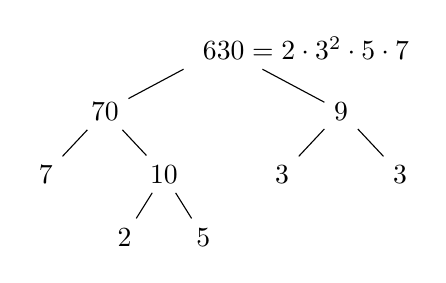
\begin{tikzpicture}[level/.style={sibling distance=30mm/#1, level distance=8mm}]
\node {$\quad \quad \quad \quad \quad \quad 630 = 2 \cdot 3^2 \cdot 5 \cdot 7$}
  child {node {70}
    child {node {7}}
    child {node {10}
      child {node {2}}
      child {node {5}}
    }
  }
  child {node {9}
    child {node {3}}
    child {node {3}}
  };
\end{tikzpicture}

\end{minipage}%
\begin{minipage}{0.40\textwidth}
 \centering
 % (c) 2014 Daniele Zambelli - daniele.zambelli@gmail.com
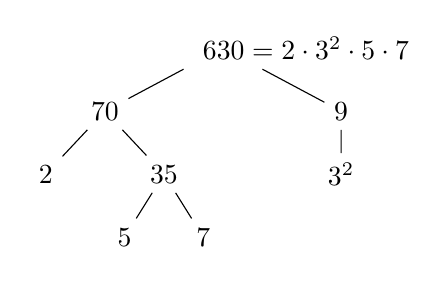
\begin{tikzpicture}[level/.style={sibling distance=30mm/#1, level distance=8mm}]
\node {$\quad \quad \quad \quad \quad \quad 630 = 2 \cdot 3^2 \cdot 5 \cdot 7$}
  child {node {70}
    child {node {2}}
    child {node {35}
      child {node {5}}
      child {node {7}}
    }
  }
  child {node {9}
    child {node {$3^2$}}
  };
\end{tikzpicture}

\end{minipage}%
\end{inaccessibleblock}

\end{exrig}

Qualunque strada si segua per scomporre un numero in fattori primi 
otterremo sempre lo stesso risultato.

\subsection{Scomposizione con un metodo sequenziale}

Possiamo anche usare un metodo sequenziale:
Sottolinea e scomponi.

\begin{exrig}
 \begin{esempio}
 Scomporre in fattori primi il numero~1260.

 $\underline{1260} = 2^{2} \cdot 3^{2} \cdot 5 \cdot 7$
 
 $\underline{10} \cdot \underline{126}$
 
 $5 \cdot 2 \cdot 2 \cdot \underline{63}$
 
 $5 \cdot 2 \cdot 2 \cdot 7 \cdot \underline{9}$
 
 $5 \cdot 2 \cdot 2 \cdot 7 \cdot 3^{2}$
 
 \end{esempio}
\end{exrig}

%\vspazio\ovalbox{\risolvi \ref{ese:1.22}, \ref{ese:1.23}, \ref{ese:1.24}}

\section{Massimo Comune Divisore e minimo comune multiplo}
\label{sec:01_mcdemcm}

\label{def:mcd}
\begin{definizione}
Il \emph{massimo comune divisore} di numeri naturali~$a$ e~$b$  è il
più grande tra tutti i divisori comuni ad~$a$ e~$b$
e si indica con~$\mcd(a,b)$,.
\end{definizione}

Applicando la definizione, il massimo comune divisore tra~18 e~12 si ottiene 
prendendo tutti i divisori di~18 e~12:
\begin{align*}
\text{divisori di }18: & \qquad 1,~2,~3,~6~9,,~18;\\
\text{divisori di }12: & \qquad 1,~2,~4,~6,~12.
\end{align*}

I divisori comuni sono~1,~2,~6, il più grande è~6, quindi:~$\mcd(18, 12)=6$. 

% \vspazio\ovalbox{\risolvi \ref{ese:1.25}}\vspazio

Per calcolare il massimo comune divisore di due o più numeri si può applicare 
la seguente procedura:

\begin{procedura}
Calcolo del~$\mcd$ di due o più numeri naturali:
\begin{enumeratea}
 \item si scompongono i numeri in fattori primi;
 \item si moltiplicano tra loro i fattori comuni, 
  presi una sola volta e con l'esponente minore .
\end{enumeratea}
\end{procedura}

% \clearpage

\begin{exrig}
 \begin{esempio}
Calcolare~$\mcd(60,48,36)$.

Si scompongono in fattori i singoli 
numeri~$60=2^2\cdot3\cdot5$,~$48=2^4\cdot3$,~$36 =2^2\cdot3^2$.
I~fattori comuni sono~2 e~3, il~2 compare con l'esponente minimo~2; 
il~3 compare con esponente minimo~1.

Pertanto~$\mcd(60,48,36)=~2^2\cdot3=12$.

 \end{esempio}

 \begin{esempio}
 Calcolare~$\mcd(60,120,90)$.

Si scompongono in fattori i singoli 
numeri~$60 =~2^2\cdot3\cdot5$,~$120 =~2^3\cdot3\cdot5$ 
e~$90=2\cdot3^2\cdot5$.
I~fattori in comune sono~2,~3,~5. L'esponente minino è~1 per tutti.

Pertanto~$\mcd(60,120,90)=~2\cdot3\cdot5=30$.
 \end{esempio}
\end{exrig}

\begin{definizione}
 Due numeri~$a$ e~$b$ si dicono \emph{primi tra loro} o \emph{coprimi} 
 se~$\mcd(a,b) =~1$.
\end{definizione}

\begin{exrig}
 \begin{esempio}
 Numeri primi tra loro:
 \begin{itemize*}
 \item 12 e~25 sono primi tra loro. Infatti il~$\mcd(12,25)=1$ dato che nelle 
  loro scomposizioni in fattori non si hanno fattori 
  comuni:~$12 =2^2\cdot3$ e~$25=5^2$;
 \item 35 e~16 sono primi tra loro. Infatti~$35=5\times~7$,~$16=2^4$. 
  I due numeri non hanno divisori comuni e il loro~$\mcd=1$;
 \item 11 e~19 sono primi tra loro infatti il~$\mcd(11,19)=1$ dato che~11 
  e~19 sono numeri primi;
 \item 12 e~15 non sono primi tra di loro in quanto hanno~3 come divisore 
  comune.
 \end{itemize*}
 \end{esempio}
\end{exrig}

\begin{definizione}
 Il \emph{minimo comune multiplo} di due numeri naturali~$a$ e~$b$ è il più
 piccolo tra tutti i multipli comuni ad~$a$ e a~$b$ 
 e si indica con~$\mcm(a,b)$.
\end{definizione}

Per calcolare il minimo comune multiplo tra~6 e~15 applicando la definizione 
occorre calcolare i primi multipli dei due numeri:
\begin{align*}
\text{multipli di }6: & \qquad~6,~12,~18,~24,~30,~36,~42,~48,~54,~60,\ldots; \\
\text{multipli di }15: & \qquad~15,~30,~45,~60,~75,~90,\ldots
\end{align*}
Sono multipli comuni~30,~60,~90,\ldots Il più piccolo dei multipli comuni è~30.

Per calcolare il minimo comune multiplo tra due o più numeri si può applicare la 
seguente procedura:

\begin{procedura}
Calcolo del~$\mcm$ di due o più numeri naturali:
\begin{enumeratea}
 \item si scompongono i numeri in fattori primi;
 \item si moltiplicano tra loro i fattori comuni e non comuni, 
  presi una sola volta, con l'esponente maggiore .
\end{enumeratea}
\end{procedura}

% \newpage

\begin{exrig}
 \begin{esempio}
 Calcolare il~$\mcm(60,48,36)$.

Scomponendo in fattori i numeri si 
ha~$60=2^2\cdot3\cdot5$;~$48=2^4\cdot3$;~$36 =2^2\cdot3^2$.
Tutti i fattori comuni e non comuni presi una sola volta con l'esponente più 
grande con cui compaiono sono:~$2^4,~3^2,~5$.

Il~$\mcm$ è~$2^4\cdot3^2\cdot5=720$.
 \end{esempio}

 \begin{esempio}
 Calcolare il~$\mcm(20,24,450)$.

Scomponendo in fattori si 
ha:~$20=2^2\cdot5$;~$24=2^3\cdot3$;~$450 =~2\cdot3^2\cdot5^2$.
Moltiplicando i fattori comuni e non comuni con il massimo esponente 
si ha~$2^3\cdot3^2\cdot5^2=1800$.
 \end{esempio}

 \begin{esempio}
 Si vuole pavimentare una stanza a pianta rettangolare di~$315\unit{cm}$ 
 per~$435\unit{cm}$ con mattonelle quadrate le più grandi possibile, 
 senza sprecarne alcuna. Quali sono le dimensioni delle 
 mattonelle? Quante mattonelle sono necessarie?

Poiché le mattonelle devono essere quadrate devono avere il lato tale che 
entri un numero intero di volte sia nel~315 sia nel~435, pertanto la 
dimensione delle mattonelle deve essere un divisore comune
di~315 e di~435. Poiché è richiesto che le mattonelle siano quanto più 
grandi possibile, la dimensione deve essere il massimo divisore comune.
\begin{center}
 % (c) 2012 Dimitrios Vrettos - d.vrettos@gmail.com
\begin{tikzpicture}[level/.style={sibling distance=20mm/#1, level 
distance=8mm}]
\node {$\quad \quad \quad \quad \quad 315 = 3^2 \cdot 5 \cdot 7$}
  child {node {5}}
  child {node {63}
    child {node {3}}
    child {node {21}
      child {node {7}}
      child {node {3}}
    }
  };
\begin{scope}[xshift=3.5cm]
\node {$\quad \quad \quad \quad \quad 435 = 3 \cdot 5 \cdot 29$}
  child {node {5}}
  child {node {87}
    child {node {3}}
    child {node {29}}
  };
\end{scope}

\begin{scope}[xshift=6cm,yshift=-4cm, scale=.8,
              every node/.style={minimum size=10mm},on grid]
    \draw[step=10mm, black, dashed] (0,0) grid (6,5);
    \fill[gray, opacity=.4] (5,4) rectangle (6,5);
    \draw[black,very thick] (0,0) rectangle (6,5);
\end{scope}
\end{tikzpicture}

% % (c) 2012 Dimitrios Vrettos - d.vrettos@gmail.com
\begin{tikzpicture}
  \begin{scope}[scale=1,every node/.style={minimum size=1cm},on grid]
    \draw[step=10mm, black, dashed] (0,0) grid (6,5);
    \fill[gray, opacity=.4] (5,4) rectangle (6,5);
    \draw[black,very thick] (0,0) rectangle (6,5);
  \end{scope} 
\end{tikzpicture}

\end{center}
La soluzione del problema è data quindi dal~$\mcd(315,435)=3\cdot5=15$. 
Le mattonelle devono avere il lato di~$15\unit{cm}$.
Ci vogliono~$435:15=29$ mattonelle per ricoprire il lato 
di~$435\unit{cm}$ e~$315:15=21$ mattonelle per ricoprire il lato
da~$315\unit{cm}$. In tutto occorrono~$29\cdot21=609$ mattonelle.
\end{esempio}
\end{exrig}

% \ovalbox{\risolvii \ref{ese:1.26}, \ref{ese:1.27}, \ref{ese:1.28}, 
% \ref{ese:1.29}, \ref{ese:1.30}, \ref{ese:1.31}, \ref{ese:1.32}}



